\chapter{Statistik}\index{Statistik|(}
\section{Grundlagen der Statistik}
Wenn klar ist, worüber wir eine Aussage machen wollen, kann man sich auf die Einzelbeobachtungen stürzen:
\begin{description}
    \item [Grundgesamtheit] \gls{symb:Omega}\index{Grundgesamtheit}
        Ist die Menge aller statistischen Einheiten(Untersuchungseinheiten) mit übereinstimmenden Identifikationskriterien (sachlich, räumlich, zeitlich).
    \item [Untersuchungseinheit] \gls{symb:omega}\index{Untersuchungseinheit}
        je nach Kontext auch Elemente, Objekte oder Individuen.
    \item [Merkmal] \index{Merkmal}
        müssen alle Elemente der Grundgesamtheit besitzen, dieses kann anschließend verglichen werden.
    \item [Ausprägung] \index{Ausprägung}
    eines Merkmals ist dann der Wert, den die Untersuchungseinheit für ein Merkmal besitzt.
\end{description}

\begin{bsp}
Eine Melone, die am 04.03.2013 von einer Obstverkäuferin angeboten wird, ist eine \textbf{Untersuchungseinheit $\omega$} aus der \textbf{Grundgesamtheit $\Omega$} der Melonen, die am selben Tag von dieser Obstverkäuferin verkauft werden.\\
Das Gewicht einer Melone ist das \textbf{Merkmal}, das jede Melone (die am 04.03.2013 von der Obstverkäuferin verkauft wird) besitzen muss. Dass die vorher beschriebene Melone das Gewicht 1kg besitzt, ist die \textbf{Ausprägung} dieses \textbf{Merkmals}.
\end{bsp}

Somit muss für jedes $\omega$ klar sein, ob $\omega\in\Omega$ oder $\omega\notin\Omega$.


\subsection{Modelle}
\begin{definition}[Statistisches Modell]:\index{statistisches Modell}\index{Modell!statistisches|see {statistisches Modell}}
Ein statistisches Modell ist eine Menge $\mathcal{P}$ von Verteilungen (siehe \ref{sec:diskrete_verteilungen} bzw. \ref{sec:stetige_verteilungen}), die für das Problem in Frage kommen.\\
Es wird unterschieden zwischen \textbf{parametrischen Modellen} und \textbf{nicht parametrischen Modellen}.
\end{definition}

\begin{description}
\item [parametrisches Modell]\index{parametrisches Modell}\index{Modell!parametrisches|see{parametrisches Modell}} Der Verteilungstyp/die Form(z.B. Alternativverteilung, Normalverteilung, usw.) ist festgelegt, jedoch die vollständige Wahrscheinlichkeitsverteilung noch nicht.\\ 
Das bedeutet, einige Eigenschaften der Verteilung können noch bestimmt und verändert werden. (z.B.: die Parameter $p$,$\mu$ und $\sigma^2$...)
\[\mathcal P=\{P_\theta, \theta\in\Theta\}\;\;\;\text{ mit }\Theta\subseteq\mathbb{R}^d\]
Wobei \gls{symb:Theta}...Parameterraum, \gls{symb:theta}...Parameter(kann Mehrdimensional sein, z.B. $\theta=\mathcal N(\mu, \sigma^2)$)

\attention{Es gibt nicht das eine ''wahre'' Modell, es gibt nur brauchbare(plausible) oder unbrauchbare Modelle. \\ Jedoch gibt es sehr wohl die ''wahre'' Verteilung mit dem ''wahren'' Parameter. Denn es wird gefordert, dass alle Parameter eindeutig festgelegte Werte besitzen.}

{
    \def\muval{1000}%TODO: evtl. die beispielwerte überdenken!!!
    \def\sigmaval{100}
\begin{bsp}\label{bsp:melonen_gewichtsverteilung}
Das Gewicht $Y$ der Melonen einer Obstverkäuferin ist Normalverteilt, $Y\sim\mathcal N(\mu, \sigma^2)$ mit unbekanntem $\mu$ und $\sigma$.

Der Parameter ist 2-dimensional: $\theta=(\mu, \sigma)$ und der Parameterraum $\Theta=\mathbb{R}\times\mathbb{R}_+$.

Ein Beispiel wäre z.B.: $\mu_0=\muval$ und $\sigma_0=\sigmaval$. (siehe Abbildung \ref{fig:melonen_gewichtsverteilung})\\
\end{bsp}
\begin{figure}
    \centering
    \begin{tikzpicture}
        {
    %note that you have to define \muval and \sigmaval before!

    \begin{axis}[
    domain=600:1400,
    axis x line=bottom, % no box around the plot, only x and y axis
    axis y line=left, % the * would suppress the arrow tips
    xtick={600,800,...,1400},
    xlabel={Gewicht [g]},
    ylabel={},%TODO: was ist diese Achse?
    samples=50,
    height=5cm,
    width=10cm,
    clip=false]

    \addplot[thin, smooth, blue] {normal_distribution(\muval,\sigmaval,x)};
    \addlegendentry[align=left]{$\mathcal{N}(\muval, \sigmaval)$};
    \draw [thick,dashed,black] (current axis.south-|{axis cs:\muval,0}) -- (current axis.north-|{axis cs:\muval,0}) node [above] {$\mu_0$};
\end{axis}
}
%Graphic
    \end{tikzpicture}
    \caption{Zu Beispiel \ref{bsp:melonen_gewichtsverteilung}: Verteilung des Gewichtes von Melonen. ($\mu_0=\muval$, $\sigma_0=\sigmaval$)}
    \label{fig:melonen_gewichtsverteilung}
\end{figure}
}

\item [nicht parametrisches Modell]\index{nicht parametrisches Modell}\index{Modell!nicht parametrisches|see{nicht parametrisches Modell}} Die Modellstruktur wird nicht von vornherein festgelegt, sondern aus den Daten bestimmt. Es bedeutet nicht, dass dieses Modell keine Parameter besitzt, sondern dass die Art und die Anzahl der Parameter flexibel und nicht von vornherein festgelegt ist. \\ ''alle'' Verteilungen sind möglich.
\end{description}



\begin{definition}[Stichprobe:$(X_1,...,X_n)$]:\index{Stichprobe}\\
Eine Stichprobe ist eine Folge von unabhängigen, identisch verteilten Zufallsvariablen mit einer (unbekannten) Verteilung $\mathcal P$. Sie ist sozusagen eine Teilmenge der Grundgesamtheit.
Der \textbf{Stichprobenumfang}\index{Stichprobenumfang} $n$ ist die Anzahl der Proben einer Grundgesamtheit.

Die Unabhängigkeit der einzelnen Stichproben erreicht man beispielsweise durch Ziehungen mit zurücklegen.
\end{definition}

\begin{definition}[Das Stichprobenmittel]\index{Stichprobenmittel}\index{Mittelwert|see{Stichprobenmittel}}\label{def:stichprobenmittel}:\\
\[\overline X_n=\sum_{i=1}^n X_i\] ist eine erwartungstreue Schätzfunktion mit $\mathbb{E}(\overline X_n)=\mu$ und $\mathbb{V}(\overline X_n)=\frac{\sigma^2}{n}$
\end{definition}
\begin{bsp} In einer Firma arbeiten 100 Personen (Grundgesamtheit=100). Davon sind 30 weiblich und 70 Männlich. Es gibt 5 Abteilungen in der Firma, in denen die Personen arbeiten.\\
Wie kann man nun Stichproben aus diesen Personen auswählen?
\begin{description}
\item [Zufällige Auswahlen]:
\begin{enumerate}[i)]
    \item Arbeiter durchnummerieren (1-100), dann 20 Zahlen zufällig ziehen.
    \item Jeder Arbeiter würfelt, bei einer 6 wird er gezogen.
    \item Eine der 5 Abteilungen wird zufällig gewählt.
\end{enumerate}
\item[Bewusste Auswahlen]:
\begin{enumerate}[i)]
    \item Bei der Betriebsversammlung die Personen wählen, auf die zufällig der Blick vom Chef fällt.
    \item Arbeiter wählen, die als erste oder letzte zur Arbeit kommen.
    \item besonders nette Arbeiter wählen.
\end{enumerate}
\end{description}
\end{bsp}

\subsection{Aufgaben der Statistik}\index{Statistik!Aufgaben}
Die Aufgabe der (induktiven/schließenden) Statistik ist es nun, auf Grund der Stichprobe $(X_1, ..., X_n)$ Aussagen über die unbekannte Verteilung bzw. der unbekannten Parameter der Grundgesamtheit $\Omega$ zu treffen.

\begin{definition}\index{Statistik!Definition}\index{Teststatistik}
eine Statistik (auch Teststatistik) $T$ ist eine Zufallsvariable, die aus einer Stichpobe berechnet wird: $T=T(X_1,...,X_n)$
\end{definition}

\subsubsection{Die Statistik besitzt 2 Grundaufgaben}
\begin{description}
    \item [Schätzen:] Aus einer Stichprobe einen Schätzwert für $\theta$ bestimmen. (+ evtl. die Genauigkeit bestimmen)
    \item [Testen:] Wenn eine Aussage über die Verteilung existiert, muss festgestellt werden, ob diese Aussage zutrifft. (gut/schlecht)
\end{description}

\section{Schätztheorie}\index{Schätztheorie}
Hierbei unterscheiden wir zwischen \textbf{Punktschätzung}\index{Punktschätzung}\index{Schätzer!Punkt-|see {Punktschätzung}} und \textbf{Intervallschätzung}\index{Intervallschätzung}\index{Schätzer!Intervall-|see {Intervallschätzung}}.
\begin{bsp}\label{bsp:schaetztheorie}
Greifen wir nochmal das Beispiel mit der Firma auf:
Beim Zählen aller Personen aus einer Abteilung(20 Personen gesamt, 6 davon sind Frauen) kommt der Statistiker auf einen Anteil der Frauen von $\theta=p=\frac{6}{20}=0.3$. 

Nimmt der Statistiker diesen beobachteten Wert ($0.3$) als $\hat\theta_n$, so hat man ein Beispiel für eine Punktschätzung.

Ist der Statistiker jedoch vorsichtiger, so könnte er diesen Wert durch ein Intervall abschätzen: $0.2\leq\hat\theta_n\leq0.4$. Oder, er sagt, dass der Frauenanteil $\hat\theta_n\geq 0.25$
\end{bsp}
\subsection{Punktschätzung}\index{Punktschätzung|(}
Die erste Aufgabe, mit der wir uns beschäftigen, besteht darin, aus einer
Stichprobe Schätzwerte für den unbekannten Parameter zu bestimmen.
Wir definieren
\begin{definition}
Ein Schätzer \gls{symb:hatthetan} ist eine Folge von Statistiken:
\[(\hat\theta_n, n\in \mathbb{N}): \hat\theta_n=\hat\theta_n(\underbrace{X_1, ..., X_n}_{Stichprobe})\;\;\Rightarrow\text{ Schätzfunktion}\]
Wobei hier $\hat\theta_n$ der Schätzwert für den Parameter $\theta$ ist.
\end{definition}
Diese Definition lässt recht dumme Schätzer zu (z.B. 42, vgl.\ Douglas
Adams), deshalb definieren wir einige wünschenswerte Eigenschaften, die wir von Schätzern erwarten:
\begin{definition}[Eigenschaften von Schätzern]:\index{Schätzer!Eigenschaften}\label{def:eigenschaften_schaetzer}
    \begin{enumerate}[i)]
        \item \textbf{Konsistenz}: \index{Konsistenz}\index{Schätzer!Konsistenz|see{Konsistenz}}$\hat\theta_n\rightarrow\theta$ für $n\rightarrow\infty$:\\
        Das bedeutet, sie ist eine Eigenschaft, die nur für große Stichprobenumfänge gilt. (D.h. eine konsistente Schätzfunktion kann für endliche Stichprobenumfänge eine große Varianz (Verzerrung) besitzen.)
        \begin{enumerate}[a)]
            \item Schätzer $\hat\theta_n$ heißt schwach konsistent, wenn $\hat\theta_n\to\theta$ in Wahrscheinlichkeit
                konvergiert (also $\lim\limits_{n\to\infty}\mathbb P_\theta(|\hat\theta_n-\theta|>\epsilon) = 0\;\;\forall\epsilon>0\;\forall\theta\in\Theta$.\\
                Das bedeutet, die Wahrscheinlichkeit, dass die Schätzfunktion $\hat\theta_n$ Werte außerhalb eines beliebig kleinen Intervalls $\epsilon$ um den wahren Wert $\theta$ annimmt, mit steigendem $n$ gegen 0 geht.\\
                (Siehe Abbildung \ref{fig:konsistenz})

            \item Schätzer $\hat\theta_n$ heißt stark konsistent, wenn $\hat\theta_n\to\theta$ mit Wahrscheinlichkeit
            1 für steigende $n$ konvergiert (also $\mathbb P_\theta(\lim\limits_{n\to\infty}|\hat\theta_n-\theta|=0)=1\;\;\forall\theta\in\Theta$).
        \end{enumerate}
        \item \textbf{Erwartungstreue, Unverzerrtheit}:\index{Erwartungstreue}\index{Schätzer!Erwartungstreue|see{Erwartungstreue}}\index{Unverzerrt}\index{Schätzer!Unverzerrtheit|see{Unverzerrtheit}}\\
            Schätzer $\hat\theta_n$ heißt erwartungstreu(unverzerrt), wenn
            \[\mathbb E_\theta(\hat \theta_n)=\theta.\]
            Also die Schätzfunktion soll gleich dem wahren Parameter $\theta$ sein.

            \textbf{Verzerrung\index{Verzerrung}(Bias)}\index{Bias}: ist definiert als $bias(\hat\theta_n)=\mathbb{E}(\hat\theta_n)-\theta$. 
            
            ($\Rightarrow$ wenn $bias(\hat\theta_n)=0$, dann ist $\hat\theta_n$ erwartungstreu.)
        \item \textbf{Effizienz:}\index{Effizienz}\index{Schätzer!Effizienz|see {Effizienz}}\\
            Schätzer $\hat\theta_n$ heißt effizient, wenn er erwartungstreu ist und die kleinste Varianz
            unter allen erwartungstreuen Schätzern hat.

            z.B: 2 Schätzer($\hat\theta_n$ und $\tilde\theta_n$): dann ist $\hat\theta_n$ effizienter, als $\tilde\theta_n$, wenn gilt:
            \[\mathbb{V}(\hat\theta_n)\leq\mathbb{V}(\tilde\theta_n)\;\;\forall\theta\]
        
    \end{enumerate}
\end{definition}
\attention{Die Eigenschaft ''\textbf{erwartungstreu}''\index{Erwartungstreue} bedeutet nicht, dass man erwarten kann, dass der Schätzer den wahren Wert liefert.
Es sagt nur, dass der Verteilungsschwerpunkt der Schätzwerte der wahre Wert $\theta$ ist und nicht systematisch abweicht.}
\begin{figure}
    \centering
    \begin{tikzpicture}
        {
\def\muval{10}
\def\sigmavalA{0.5}
\def\sigmavalB{0.8}
\def\sigmavalC{1.2}
\def\epsilonval{1}
\def\beginval{6}
\def\endval{14}

\pgfmathsetmacro{\muPlusEps}{\muval+\epsilonval}
\pgfmathsetmacro{\muMinusEps}{\muval-\epsilonval}

\begin{axis}[
    domain=\beginval:\endval,
    axis x line=bottom, % no box around the plot, only x and y axis
    axis y line=left, % the * would suppress the arrow tips
    xtick={6,8,...,14},
    samples=50,
    height=5cm,
    width=10cm,
    clip=false
]

% Fill curve-part right
\addplot [
    fill=black!50,
    draw=none,
    forget plot,            %prevent from listing in legend
    domain=\muPlusEps:\endval
] {normal_distribution(\muval,\sigmavalC,x)} \closedcycle;
\addplot [
    fill=blue!60,
    draw=none,
    forget plot,            %prevent from listing in legend
    domain=\muPlusEps:\endval
] {normal_distribution(\muval,\sigmavalB,x)} \closedcycle;
\addplot [
    fill=green!60,
    draw=none,
    forget plot,            %prevent from listing in legend
    domain=\muPlusEps:\endval
] {normal_distribution(\muval,\sigmavalA,x)} \closedcycle;

% Fill curve-part left
\addplot [
    fill=black!50,
    draw=none,
    forget plot,            %prevent from listing in legend
    domain=\beginval:\muMinusEps
] {normal_distribution(\muval,\sigmavalC,x)} \closedcycle;
\addplot [
    fill=blue!60,
    draw=none,
    forget plot,            %prevent from listing in legend
    domain=\beginval:\muMinusEps
] {normal_distribution(\muval,\sigmavalB,x)} \closedcycle;
\addplot [
    fill=green!60,
    draw=none,
    forget plot,            %prevent from listing in legend
    domain=\beginval:\muMinusEps
] {normal_distribution(\muval,\sigmavalA,x)} \closedcycle;


% Draw curves
\addplot [thin, smooth, color=green, name path global=first] {normal_distribution(\muval,\sigmavalA,x)};
\addlegendentry[align=left]{$\hat\theta_a$}
\addplot [thin, smooth, color=blue, name path global=second] {normal_distribution(\muval,\sigmavalB,x)};
\addlegendentry{$\hat\theta_b$}
\addplot [thin, smooth, color=black, name path global=second] {normal_distribution(\muval,\sigmavalC,x)};
\addlegendentry{$\hat\theta_c$}
% Draw vertical line:
\draw [dashed, black, thick] (current axis.south-|{axis cs:\muval,0}) -- (current axis.north-|{axis cs:\muval,0})node [above] {$\theta$};
\draw [red, thick, name intersections={of={first and second}}] (current axis.north-|{axis cs:\muPlusEps,0}) -- (current axis.south-|{axis cs:\muPlusEps,0}) node [below] {$\theta+\epsilon$};
\draw [red, thick, name intersections={of={first and second}}] (current axis.north-|{axis cs:\muMinusEps,0}) -- (current axis.south-|{axis cs:\muMinusEps,1}) node [below] {$\theta-\epsilon$};
\end{axis}
}

    \end{tikzpicture}
    \caption{Konsistenz der einzelnen Schätzer $\hat\theta_a$, $\hat\theta_b$ und $\hat\theta_c$, wobei für die Stichprobenumfänge gilt: $a>b>c$}
    \label{fig:konsistenz}
\end{figure}


\subsubsection{Momentenmethode}\index{Momentenmethode|(}\index{Schätzer!Momentenschätzer|see{Momentenmethode}}
Eine einfache Methode, um Schätzer zu konstruieren, ist die Momentenmethode\index{Momentenmethode}\index{Schätzer!Momentenschätzer|see{Momentenmethode}}. Mit ihr kann man die unbekannten Komponenten des Parametervektors $\vec\theta=(\theta_1,\theta_2,...,\theta_k)$ bestimmen.

Ihr liegt das Gesetz der großen Zahlen zugrunde. Diese Methode ist sehr einfach, jedoch sind die resultierenden Schätzer nicht immer Erwartungstreu. \\

\begin{definition}[Moment]:\index{Moment}\label{def:moment}\\
    Das Moment der Ordnung $k$ von $X$(wobei $X$ eine Zufallsvariable ist) ist wie folgt definiert:
    \[m_k=\mathbb{E}(X^k)\;\;\forall k\in\mathbb{N}\]
    Das $k$-te Moment von $X$ ist sozusagen der Erwartungswert der $k$-ten Potenz von $X$.
\end{definition}

\textbf{Vorgangsweise, um $k$ unbekannte Parameter $\vec\theta$ zu berechnen:}
    Die ersten $k$-Momente der Verteilung können als Funktion der Parameter $\vec\theta=(\theta_1,\theta_2,...,\theta_k)$ ausgedrückt werden:
        \[\mathbb{E}(X^j)=m_j=g_j(\theta_1, \theta_2, ..., \theta_k)\;\;\forall j=1,...,k\text{ bzw. }\]
        \[\mathbb{E}(X^j)=m_j=g_j(\vec\theta)\;\;\forall j=1,...,k\]
        Die \textbf{empirischen Momente}\index{Moment!empirisches}\index{empirisches Moment}
        \[\hat m_j=\frac{1}{n}\sum_{i=1}^n x_i^j\;\;\forall j=1,...,k\]
        können anschließend für die Momente $m_j\;\;\forall j=1,...,k$ eingesetzt werden: (dabei wird aus dem Parametervektor $\vec\theta$ der Schätzervektor $\vec{\hat{\theta_n}}$.)
        \[g_j(\vec{\hat{\theta_n}})=\frac{1}{n}\sum_{i=1}^n x_i^j=\mathbb{E}(X^j)\;\;\forall j=1,...,k\]
        \[\vec{\hat{\theta_n}}=g_j^{-1}\left(\frac{1}{n}\sum_{i=1}^n x_i^j\right)=g_j^{-1}(\mathbb{E}(X^j))\;\;\forall j=1,...,k\]
        Damit hat man ein Gleichungssystem mit $k$-Gleichungen, die gelöst werden müssen.

\begin{bsp}
Angenommen, $\Omega$ ist Poissonverteilt ($\mathcal P(\lambda)$): $\Rightarrow\mathbb{E}(X)=\lambda$.\\
D.h. nur ein Parameter $\lambda$ ist zu berechnen, folglich ist unser $k=1$:
\[\theta_1=\lambda=\mathbb{E}(X)=m_1\;\;\text{ und }\;\;\hat m_1=\frac{1}{n}\sum_{i=1}^n x_i\]
\[\Rightarrow \hat\theta_n=\hat\lambda=\frac{1}{n}\sum_{i=1}^nx_i\]
\end{bsp}

\begin{bsp}
Angenommen, $\Omega$ ist Normalverteilt ($N(\mu, \sigma^2)$): \\
$\Rightarrow\mathbb{E}(X)=\mu$ und $\sigma^2=\mathbb{E}(X^2)-\mathbb{E}(X)^2$.\\
Da die Normalverteilung 2 Parameter ($\mu$ und $\sigma$) besitzt, ist unser $k=2$:
\[\text{Mit }\;\;\theta_1=\mu=\mathbb{E}(X)=m_1\;\;\text{ und }\;\;\hat m_1=\frac{1}{n}\sum_{i=1}^n x_i\;\;\;\;\Rightarrow\;\;\hat\theta_1=\hat\mu=\frac{1}{n}\sum_{i=1}^nx_i\]
\[\text{Mit }\;\;\theta_2=\mathbb{E}(X^2)=m_2\;\;\text{ und }\;\;\hat m_2=\frac{1}{n}\sum_{i=1}^n x_i^2\;\;\;\;\Rightarrow\;\;\hat\theta_2=\frac{1}{n}\sum_{i=1}^nx_i^2\]
\[\Rightarrow \hat\sigma^2=\hat\theta_2+(\hat\theta_1)^2=\frac{1}{n}\sum_{i=1}^nx_i^2+{\underbrace{\left(\frac{1}{n}\sum_{i=1}^nx_i\right)}_{\overline{x_n}}}^2=\frac{1}{n}\sum_{i=1}^nx_i^2+\overline{x_n}^2\]
\end{bsp}


\subsubsection{Maximum Likelihood Methode}\index{Maximum Likelihood Methode|(}
Eine andere Methode um Schätzer zu konstruieren, ist die Maximum Likelihood Methode:

{
    \def\nval{20}
    \def\kval{6}
\begin{bsp} Fortsetzung zu Beispiel \ref{bsp:schaetztheorie}
    \label{bsp:binomial_probability}
nehmen wir an, die Anzahl der weiblichen Arbeiter $Y$ ist Binomialverteilt ($Y\sim B_n(\theta)$) mit Parameter $\theta$. \\
Wie wahrscheinlich ist es nun, im Modell der Binomialverteilung, den beobachteten Wert $k=\kval$ zu erhalten?
\[P_\theta(Y=k)=\binom{n}{k}\theta^k(1-\theta)^{n-k}\;\;\Rightarrow\;\;P_\theta(Y=6)=\binom{\nval}{\kval}\theta^\kval(1-\theta)^{\nval-\kval}\]
Siehe Abbildung \ref{fig:binomial_probability}, hier sieht man, dass die Wahrscheinlichkeit, dass der Anteil der Frauen $\theta=0.3$ beträgt, am höchsten ist (rote Linie) mit $P_{0.3}(Y=\kval)=\binomialDistributionValue{\nval}{\kval}{0.3}$.

Bei $\theta=0.4$ (grün) ist $P_{0.4}(Y=\kval)=\binomialDistributionValue{\nval}{\kval}{0.4}$ und bei $\theta=0.5$ ist $P_{0.5}(Y=\kval)=\binomialDistributionValue{\nval}{\kval}{0.5}$, d.h. die Wahrscheinlichkeit ist immer noch relativ groß. 

Erst bei $\theta=0.6$ ist die Wahrscheinlichkeit $P_{0.6}(Y=\kval)=\binomialDistributionValue[4]{\nval}{\kval}{0.6}$ ein kleiner Bruchteil von $P_{0.3}$.

\end{bsp}
\begin{figure}
     \centering
    \begin{tikzpicture}
        {
    %note that you have to define \nval and \kval before!

    \pgfmathtruncatemacro{\nvalB}{\nval*3}%save \nval*3 without floating-points to \nvalB

    \pgfmathtruncatemacro{\kvalB}{\kval*3}

    \begin{axis}[
    domain=0:1,
    ymax=0.21,%otherwise the intersection-point on theta=0.3 would fail
    yticklabel style={/pgf/number format/fixed},%to prevent a axis-entry like 5*10^-2
    axis x line=bottom, % no box around the plot, only x and y axis
    axis y line=left, % the * suppresses the arrow tips
    xtick={0.1,0.2,...,1},
    xlabel={$\theta$},
    ylabel={$P_\theta(Y=k)$},
    samples=50,
    height=5cm,
    width=10cm,
    clip=false]

    \addplot[name path global=plot,thin, smooth, blue] {binomial_distribution(\nval,\kval,x)};
    \addplot[name path global=plot2,thin, smooth, orange] {binomial_distribution(\nvalB,\kvalB,x)};
    \addlegendentry[align=left]{$\mathcal{B}_{\nval,\kval}(\theta)$};
    \addlegendentry[align=left]{$\mathcal{B}_{\nvalB,\kvalB}(\theta)$};


    %find intersection with binomial_distribution on theta=0.3
    \node[coordinate] (Ref) at (axis cs:0.3,0) {};
    \path[name path global=RefPath] (Ref |- current axis.south) -- (Ref |- current axis.north);
    \path [name intersections={of=plot and RefPath}];
    \coordinate (I1)  at (intersection-1);
    %draw line to intersection on theta=0.3
    \draw [ultra thick,dashed,red] ({rel axis cs:0,0}-|Ref) -- (I1);


    %find intersection with binomial_distribution on theta=0.4
    \node[coordinate] (Ref) at (axis cs:0.4,0) {};
    \path[name path global=RefPath] (Ref |- current axis.south) -- (Ref |- current axis.north);
    \path [name intersections={of=plot and RefPath}];
    \coordinate (I2)  at (intersection-1);
    %draw line to intersection on theta=0.3
    \draw [ultra thick,dashed,green] ({rel axis cs:0,0}-|Ref) -- (I2);


    %find intersection with binomial_distribution on theta=0.5
    \node[coordinate] (Ref) at (axis cs:0.5,0) {};
    \path[name path global=RefPath] (Ref |- current axis.south) -- (Ref |- current axis.north);
    \path [name intersections={of=plot and RefPath}];
    \coordinate (I3)  at (intersection-1);
    %draw line to intersection on theta=0.5
    \draw [ultra thick,dashed,brown] ({rel axis cs:0,0}-|Ref) -- (I3);
\end{axis}
}
%Graphic
    \end{tikzpicture}
    \caption{Zu Beispiel \ref{bsp:binomial_probability}: Zeigt die Wahrscheinlichkeiten $P_\theta(Y=\kval)$ für die einzelnen $\theta$-Werte. ($\mathcal{B}_{\nval,\kval}$). Außerdem sieht man, dass die Wahrscheinlichkeit bei einer 3x größeren Stichprobe($n=\nval\cdot3$ und $k=\kval\cdot 3$) nicht mehr so stark streut. ($\mathcal{B}_{\nval\cdot 3,\kval\cdot 3}$)}
    \label{fig:binomial_probability}
\end{figure}
}

Wenn die Wahrscheinlichkeit, die aktuelle Zufallsvariable(Ereignis) zu erhalten,
für einen Parameter sehr klein ist, spricht das gegen diesen Parameter.
Umgekehrt heißt das, dass ein Parameterwert umso plausibler ist, je größer
die Wahrscheinlichkeit der Zufallsvariable unter diesem Parameter ist. 

Hier kommt nun die Likelihood-Funktion ins Spiel:
\begin{definition}\index{Likelihood-Funktion}Die Likelihoodfunktion für eine diskrete Zufallsvariable(Ereignis) X, mit gegebendem Modell(Verteilung), abhängig von Parameter $\theta\in\Theta$ ist definiert als:\label{def:likelihoodfunktion}
\[L(X;\theta)=c(X)\cdot P_\theta(X)\]
und für stetige Zufallsvariablen X mit der Dichte $f_\theta(X)$ folgt:
\[L(X;\theta)=c(X)\cdot f_\theta(X)\]
\end{definition}
Das \textbf{Likelihood-Prinzip}\index{Likelihood-Prinzip}: Berechne die Wahrscheinlichkeit, genau die Stichprobe $\omega$ aus $\Omega$ zu ziehen.

Wobei $c(X)$ ein konstanter Faktor ist, der NICHT von $\theta$ abhängt. $\Rightarrow$ die Likelihood-Funktion ist mehrdeutig.

\begin{definition}\index{Likelihood-Funktion!Log-|see{Log-Likelihood-Funktion}}\index{Log-Likelihood-Funktion}
Die Log-Likelihood-Funktion ist wie folgt definiert:
\[l(X;\theta)=\ln\,L(X;\theta)\]
sie wird häufig verwendet, denn sie ist meist viel handlicher.
\end{definition}

\begin{definition}Multiplikationssatz für Likelihood-Funktionen:\index{Likelihood-Funktion!Multiplikationssatz|see{Multiplikationssatz für Likelihood-Funktionen}}\index{Multiplikationssatz für Likelihood-Funktionen}\label{def:multiplikationssatz_likelihood}

Die Stichprobe $\vec X=(X_1, X_2, ..., X_n)$ setzt sich aus $n$ unabhängigen Zufallsvariablen(Ereignissen) zusammen:
    \[L(\vec X;\theta) = L(X_1, X_2, ..., X_n;\theta) = \prod_{i=1}^nL(X_i;\theta)\]
somit gilt für die Log-Likelihood-Funktion:
    \[l(\vec X;\theta) = l(X_1, X_2, ..., X_n;\theta) = \sum_{i=1}^nl(X_i;\theta)\]
\end{definition}

\begin{bsp}\label{bsp:likelihood}
Ein Mitarbeiter wurde beauftragt, den Anteil $\theta$ der weiblichen Arbeiter zu schätzen. Dazu schreibt er sich zu jeder Person $X_i$ auf, ob diese männlich ($X_i=0$), oder weiblich ($X_i=1$) war.

Um den Anteil nun zu bestimmen, hat er sich die 20 Personen aus der Selben Abteilung wie in Beispiel \ref{bsp:binomial_probability} angesehen und folgende Überlegung gemacht:
Da jede Person die gleiche Wahrscheinlichkeit besitzt, gilt folgendes:
\[L(X_i=1;\theta)=P(X_i=1;\theta)=\theta\]
\[L(X_i=0;\theta)=P(X_i=0;\theta)=1-\theta\]

Die Stichprobe lautet wie folgt: \[\vec\omega = \{X_1=1, X_2=0, X_3=1, X_4=0,X_5=0,X_6=0,X_7=1,X_8=1,\]
    \[X_9=0,X_{10}=0,X_{11}=0,X_{12}=0,X_{13}=0,X_{14}=1,X_{15}=0,\]
    \[X_{16}=0,X_{17}=0,X_{18}=0,X_{19}=1,X_{20}=0\} \]
Mit dem Multiplikationssatz (siehe Definition \ref{def:multiplikationssatz_likelihood}) gilt nun:
\begin{eqnarray*}
L(\vec\omega;\theta)&=&L(X_1=1;\theta)\cdot L(X_2=0;\theta)\cdot ...\cdot L(X_{20}=0;\theta)\\
L(\vec\omega;\theta)&=&(1-\theta)\cdot \theta \cdot (1-\theta)\cdot ... \cdot \theta \cdot (1-\theta)=\theta^6\cdot(1-\theta)^{14}\\
\end{eqnarray*}
Das ist aber wiederum das selbe Ergebnis, wie das aus Beispiel \ref{bsp:binomial_probability}, bis auf den konstanten Faktor $\binom{20}{6}$, dieser ist aber nicht so wichtig, denn die Likelihood-Funktion ist, wie bereits erwähnt mehrdeutig.
\end{bsp}


Und nun kommen wir zum Maximum-Likelihood-Schätzer:

\begin{definition}\index{Maximum-Likelihood-Schätzer}\index{ML-Schätzer|see{Maximum-Likelihood-Schätzer}}\index{Schätzer!Maximum-Likelihood-|see{Maximum-Likelihood-Schätzer}}
Der Maximum-Likelihood (ML-) Schätzer $\hat\theta_n$ ist der Wert von $\theta$, der die Likelihoodfunktion im Parameterraum $\Theta$ maximiert:

\[L(X,\hat\theta_n)\geq L(X,\theta)\;\;\forall \theta\in\Theta\]
\end{definition}

Der ML benötigt das Maximum der Likelihood-Funktion, somit müssen wir $L(X;\theta)$ einmal ableiten, um das Maximum zu erhalten.
Meist ist es aber einfacher, statt der Likelihood-Funktion die Log-Likelihood-Funktion $l(X;\theta)$ zu verwenden.

\begin{bsp}\label{bsp:likelihood_2}
Fortsetzung von Beispiel \ref{bsp:likelihood}: (Log-Produktregeln siehe Anhang \ref{sec:logarithmus_produkte})
\[L(\vec\omega;\theta)=\theta^6\cdot(1-\theta)^{14}\;\;\Rightarrow\;\;l(\vec\omega;\theta)=\ln(\theta^6\cdot (1-\theta)^{14})=6\cdot \ln(\theta)+14\cdot \ln(1-\theta)\]
\[\frac{dl(\vec\omega;\theta)}{d\theta}=l'(\vec\omega;\theta)=\frac{6}{\theta}+\frac{14}{1-\theta}(-1)\]
Da $l(\vec\omega;\theta)$ am Maximum ($\theta=\hat\theta_n$) die Steigung=$0$ besitzt, folgt:
\[l'(\vec\omega;\hat\theta_n)=0=\frac{6}{\hat\theta_n}+\frac{14}{1-\hat\theta_n}(-1)\;\;\Rightarrow\;\;\frac{6}{\hat\theta_n}=\frac{14}{1-\hat\theta_n}\;\;\Rightarrow\;\;6-6\hat\theta_n=14\hat\theta_n\;\;\Rightarrow\;\;20\hat\theta_n=6\]
\[\hat\theta_{20}=\frac{6}{20}=0.3\]
Das ist auch genau das, was man erwartet, wenn in einer Stichprobe mit dem Umfang $20$ sechs Elemente die Ausprägung weiblich besitzen.
\end{bsp}

\begin{bsp}\label{bsp:ml_normalverteilung}
    Gesucht sind $\mu$ und $\sigma$ der Normalverteilung $\mathcal N(\mu, \sigma^2)$ mittels Maximum-Likelihood-Schätzer: 

    Die Dichte der Normalverteilung ist ja wie folgt definiert, als 
    
    \[f_{\mu,\sigma}(x_i)=\frac{1}{\sigma\sqrt{2\pi}}e^{-\frac{(y_i-\mu)^2}{2\sigma^2}}\]
    ohne der Konstante $\frac{1}{\sqrt{2\pi}}$ erhalten wir für den Log-Likelihood:
    \[l(x_i;\mu, \sigma)=\ln\left(\frac{1}{\sigma}e^{-\frac{(y_i-\mu)^2}{2\sigma^2}}\right)=
    \ln\left(\sigma^{-1}\right)+\ln\left(e^{-\frac{(y_i-\mu)^2}{2\sigma^2}}\right)=
    -\ln\sigma-\frac{(y_i-\mu)^2}{2\sigma^2}\]
    Somit gilt für $\vec x=(x_1, ..., x_n)$:
    \[l(\vec x;\mu, \sigma)=\sum_{i=1}^nl(x_i;\mu,\sigma)=
    \sum_{i=1}^n\left(-\ln\sigma-\frac{(y_i-\mu)^2}{2\sigma^2}\right)=
    -n\cdot \ln\sigma-\frac{1}{2\sigma^2}\sum_{i=1}^n(y_i-\mu)^2
    \]
    Mit dem Steinerschen Verschiebungssatz (siehe Satz \ref{satz:steinerscher_verschiebungssatz})folgt:
    \[\mathbb E((X-a)^2)=\mathbb V(X)+(\mathbb E(X)-a)^2\;\;\Rightarrow\;\;\frac{\sum_{i=1}^n((X-a)^2)}{n}=\mathbb V(X)+(\frac{\sum_{i=1}^n(X)}{n}-a)^2\]
    \[{\sum_{i=1}^n((y_i-\mu)^2)}=n\cdot\mathbb V(\vec y)+n\cdot(\frac{\sum_{i=1}^n(y_i)}{n}-\mu)^2=
    n\cdot\mathbb V(\vec y)+n\cdot(\overline y-\mu)^2
    \]
    Somit erhalten wir: 
    \[l(\vec x;\mu, \sigma)=
    -n\cdot \ln\sigma-\frac{n}{2\sigma^2}\left(\mathbb V(\vec y)+(\overline y-\mu)^2\right)
    \]
    Zum bestimmen des ML-Schätzers müssen wir Differenzieren:\\
    Bestimmen von $\hat\mu$:
    \[\frac{\partial l(\vec x;\mu, \sigma)}{\partial \mu}=
    \frac{\partial \left(-n\cdot \ln\sigma-\frac{n\mathbb{V}(\vec y)}{2\sigma^2}+\frac{n\cdot(\overline y-\mu)^2}{2\sigma^2}\right)}{\partial \mu}=
    \frac{\cancel2\cdot n\cdot(\overline y-\mu)}{\cancel 2\sigma^2}=0
    \]
    Umformen auf $\mu$:
    \[\overline y-\mu=0\;\;\Rightarrow\;\;\overline y=\hat\mu\]

    Bestimmen von $\hat\sigma$:
    \[\frac{\partial l(\vec x;\mu, \sigma)}{\partial \sigma}=
    \frac{\partial \left(-n\cdot \ln\sigma-\frac{n\mathbb{V}(\vec y)}{2\sigma^2}+\frac{n\cdot(\overline y-\mu)^2}{2\sigma^2}\right)}{\partial \sigma}=\frac{-n}{\sigma}+\frac{n}{2}2\sigma^{-3}\left(\mathbb V(\vec y)+(\overline y-\mu)^2\right)
    =0\]
    Umformen auf $\sigma$:
    \[\frac{\cancel n}{\sigma^3}\left(\mathbb V(\vec y)+(\overline y-\mu)^2\right)
    =\frac{\cancel n}{\sigma}\;\;\Rightarrow\;\;
    \left(\mathbb V(\vec y)+(\overline y-\mu)^2\right)
    =\sigma^2\;\;\Rightarrow\;\;
    \hat\sigma=\sqrt{\left(\mathbb V(\vec y)+(\overline y-\mu)^2\right)}\]
    Eingesetzt für $\mu=\hat\mu=\overline y$ folgt:
    \[
    \hat\sigma=\sqrt{\left(\mathbb V(\vec y)+(\overline y-\overline y)^2\right)}=\sqrt{\left(\mathbb V(\vec y)\right)}\]

    Somit sind bei der Normalverteilung der Mittelwert und die Wurzel aus der Varianz die Maximum Likelihood Schätzer für $\mu$ und $\sigma$.
    \[\hat \mu=\overline y\text{ und }\hat \sigma=\sqrt{\mathbb{V}(y)}\]
\end{bsp}


\index{Maximum Likelihood Methode|)}

Damit der ML-Schätzer konsistent ist, müssen die Dichten gewisse Regularitätsvoraussetzungen erfüllen.
Bei der Suche nach einem effizienten Schätzer hilft der
\begin{satz}[Cramér-Rao]\index{Cramér-Rao, Satz}\index{Satz von Cram\'er-Rao|see{Cramér-Rao, Satz}}\label{satz:cramer_rao}
Wenn $p_\theta$ bzw.\ $f_\theta$ zweimal nach $\theta$ differenzierbar ist
und zusätzliche Regularitätsvoraussetzungen erfüllt, dann gilt für
jeden \textbf{Erwartungstreuen} Schätzer $\hat\theta_n$
\[\mathbb V(\hat\theta_n)\ge {1\over I_n(\theta)}={1\over nI(\theta)}.\]
D.h. sie liefert eine untere Schranke für die Varianz eines Schätzers $\hat\theta_n$ bzgl. des zu schätzenden Parameters $\theta$.
Dabei ist
\[I_n(\theta)=-\mathbb E_\theta\left({\partial^2\over\partial\theta^2}\log
(L(X_1,\dots,X_n;\theta))\right)\]
die \textbf{Fisher-Information}.

Wenn die Cramér-Rao-Schranke angenommen wird, ist der ML-Schätzer effizient.
\end{satz}

\begin{definition}\index{Fisher-Information}Die \textbf{Fischerinformation} ist für stetige Zufallsvariablen $X$ mit der Dichte $f_\theta(X)$ definiert ist, als
\[I(\theta)=-\mathbb E_\theta\left({\partial^2\over\partial\theta^2}\log
(f_\theta(X))\right)\]
bzw. für diskrete Zufallsvariablen $X$ definiert ist, als
\[I(\theta)=-\mathbb E_\theta\left({\partial^2\over\partial\theta^2}\log
(p_\theta(X))\right).\]
\end{definition}
Da die Log-Likelihood wie folgt definiert ist, 
\[\ln L(\vec X;\theta)=\sum_{i=1}^n \ln(p_\theta(x)\]
folgt außerdem:
\begin{eqnarray*}
I_n(\theta) &=& -\mathbb E_\theta\left({\partial^2\over\partial\theta^2}\ln
(L(\vec X;\theta))\right) = -\mathbb E_\theta\left({\partial^2\over\partial\theta^2}\sum_{i=1}^n \ln(p_\theta(X))\right)= \\
I_n(\theta) &=& -\sum_{i=1}^n \mathbb E_\theta\left({\partial^2\over\partial\theta^2}\ln(p_\theta(X))\right) = -n\cdot\underbrace{\mathbb E_\theta({\partial^2\over\partial\theta^2}\ln(p_\theta(X)))}_{I(\theta)}=-n\cdot I(\theta)
\end{eqnarray*}

Wenn wir einen erwartungstreuen 
Schätzer finden können, dessen Varianz mit der
Cram\'er-Rao Schranke übereinstimmt, dann können wir sicher sein, dass
er effizient ist. 

Allerdings gibt es einen solchen Schätzer nicht immer, 
die Dichte bzw.\ Wahrscheinlichkeitsfunktion muss dazu von einer bestimmten
Form sein. Wenn es einen solchen Schätzer gibt, dann stimmt er mit
dem Maximum-Likelihood Schätzer überein (überhaupt ist der ML-Schätzer
unter gewissen Regularitätsvorraussetzungen asymptotisch normalverteilt
mit Mittel $\theta$ und Varianz $1/I_n(\theta)$, also gewissermaßen
``asymptotisch effizient'').

\begin{bsp}
Gehen wir wieder zurück zur Obstverkäuferin von Beispiel \ref{bsp:melonen_gewichtsverteilung}

Hier hatten wir das Gewicht $Y$ der Melonen Normalverteilt. ($Y=\mathcal N(\mu, \sigma^2)$)
Gehen wir davon aus, dass wir das $\sigma^2$ bereits kennen und $\hat\mu_n$ mit $\hat\mu_n=\overline X_n$ abschätzen.

Wir sollen nun herausfinden, ob der Schätzer effizient ist: (Siehe Normalverteilung, Dichtefunktion \ref{sec:normalverteilung})

Lt. Definition \ref{def:stichprobenmittel} ist das Stichprobenmittel ein erwartungstreuer Schätzer, daher können wir den Cramér-Rao-Satz anwenden.

\[f(x,\mu)=\frac{1}{\sqrt{2\pi\sigma^2}}\cdot e^{-\frac{(x-\mu)^2}{2\sigma^2}}\Rightarrow\]
\[\ln f(x,\mu)=\ln\left(\frac{1}{\sqrt{2\pi\sigma^2}}\cdot e^{-\frac{(x-\mu)^2}{2\sigma^2}}\right)=
\ln\left(\frac{1}{\sqrt{2\pi\sigma^2}}\right)+ \left(-\frac{(x-\mu)^2}{2\sigma^2}\right)\underbrace{\ln(e)}_{=1}
\]
Bildung der 2 Ableitungen:
\[\frac{\partial \ln f(x,\mu)}{\partial\mu}=-\frac{\cancel 2(x-\mu)(-1)}{\cancel 2\sigma^2}=\frac{x-\mu}{\sigma^2}\]
\[\frac{\partial^2 \ln f(x,\mu)}{\partial\mu^2}=-\frac{1}{\sigma^2}\;\;\Rightarrow\;\;I(\mu)=\frac{1}{\sigma^2}\]
Folglich ist die Cramér-Rao-Schranke definiert als: $\mathbb{V}(\hat\mu_n)\geq \frac{\sigma^2}{n}$.

Da $\mathbb V(\overline X_n)=\frac{\sigma^2}{n}$ in Definition \ref{def:stichprobenmittel} definiert wurde, folgt:

$\mathbb V(\hat\mu_n)=\mathbb V(\overline X_n)=\frac{\sigma^2}{n}\;\;\Rightarrow\;\;\hat\mu_n\text{ ist effizient für }\mu$ 
\end{bsp}

\begin{definition}\index{suffizient}
Eine Statistik $T=T(X_1,...,X_n)$ heißt suffizient, wenn die bedingte Verteilung von $(X_1,..., X_n)$ unter $T$ nicht von $\theta$ abhängt.

Wenn die Likelihood-Funktion in der Form 
\[L(X_1,...,X_n;\theta)=g(T,\theta)\cdot h(X_1,...,X_n)\]
geschrieben werden kann, dann ist $T$ suffizient.
\end{definition}

\begin{bsp}
Nehmen wir wieder das Beispiel mit den weiblichen Arbeitern \ref{bsp:likelihood_2}:
diese sind, wie bereits erwähnt, Binomialverteilt (siehe Kapitel \ref{sec:binomialverteilung}), d.h.
Die Wahrscheinlichkeit $k$ weibliche Arbeiter bei einer Stichprobengröße von $n$ zu erhalten beträgt (wie ebenfalls bereits erwähnt):
\[p_\theta(X=k)=\binom{n}{k}\cdot \theta^k(1-\theta)^{n-k}\;\;\Rightarrow\;\;L(\vec X;\theta)=\theta^k(1-\theta)^{n-k}\text{...($p_\theta$ ohne konst. Faktoren)}\]
Da die Zufallsvariablen $X_1,...,X_n$ nur $1$(weiblich), oder $0$(männlich) sein können, folgt:
\[L(\vec X;\theta)=\theta^{\sum_{i=1}^nX_i}(1-\theta)^{n-{\sum_{i=1}^nX_i}}\]
Setzt man nun $T=T(X_1,...,X_n)=\sum_{i=1}^nX_i$, folgt: 
\[L(\vec X;\theta)=\underbrace{\theta^T(1-\theta)^{n-T}}_{g(T,\theta)}\]
{\color{red}lt. definition sollte die funktion $T(X_1,...,X_n)$ ja eig. auch eine h-Funktion besitzen, ist dieser hier 1? man weiß es nicht...?}
%TODO: lt. definition sollte die funktion T(X_1,...,X_n) ja eig. auch eine h-Funktion besitzen, ist dieser hier 1? man weiß es nicht...
Daher ist $T=T(X_1,...,X_n)=\sum_{i=1}^nX_i$ suffizient für $\theta$.
\end{bsp}

\begin{bsp}
Unsere Stichprobe $\vec\omega = X_1, ..., X_n$ ist Poissonverteilt, existiert eine Wahrscheinlichkeitsfunktion, die in $h(X_1,...,X_n)$ und $g(T, \theta)$ zerlegt werden kann, so dass $T(X_1, ..., X_n)$ eine suffiziente Statistik bildet?

\[p_\theta(x_i)=\frac{\theta^x\cdot e^{-\theta}}{x!}\;\;\Rightarrow\;\;L(\vec\omega;\theta)=
\prod_{i=1}^np_\theta(x_i)=\prod_{i=1}^n\frac{\theta^{x_i}\cdot e^{-\theta}}{x_i!}=
\underbrace{\prod_{i=1}^n\frac{1}{x_i!}}_{h(X_1,...,X_n)}\cdot\underbrace{\theta^{\sum_{i=1}^n x_i}\cdot e^{-\theta}}_{g(\sum_{i=1}^n x_i,\theta)}\]
Somit ist $T=\sum_{i=1}^n x_i$ suffizientsuffizient.
\end{bsp}

\begin{satz}
wenn die Dichten-/Wahrscheinlichkeitsfunktionen ''brav'' sind, dann ist Maximum-Likelihood-Schätzer konsistent. (Wenn noch etwas ''braver'', dann gilt: $\hat\theta_n\approx\mathcal{N}\left(\theta,\frac{1}{nI(\theta)}\right)$)

d.h. für große $n$ ist der ML-Schätzer approximativ nromalverteilt.
\end{satz}

Für wichtige Verteilungen kann man mit den genannten Kriterien gute/optimale Schätzer generieren, allerdings passen sie nur für diese Verteilungsmodelle, auf die sie zugeschnitten sind. In der Praxis sind die Modelle aber immer etwas anders. Folglich nimmt man oft weniger effiziente Schätzer, aber dafür sind die auch nicht so anfällig bei anderen Modellen. Sie werden als \textbf{robuste Schätzer}\index{robuster Schätzer}\index{Schätzer!robus|see{robuste Schätzer}} bezeichnet.

\index{Punktschätzung|)}

\subsection{Intervallschätzung}\index{Intervallschätzung|(}
Die Punkschätzer sind präzise, aber auch meist falsch. Wenn z.B.: der Schätzer $\hat\theta_n$ eine stetige Zufallsvariable ist, so ist $P(\hat\theta_n=\theta)=0$. D.h. man verliert jede Sicherheit.

Manchmal möchte man aber auch Angaben über die Genauigkeit eines Schätzwertes
machen können, also ein Intervall bestimmen, in dem der gesuchte Parameter
liegt. Leider kann so etwas nicht mit absoluter Sicherheit geschehen, weil
in den meisten Fällen für jeden Wert des Parameters jede Stichprobe
positive (wenn auch sehr kleine) Wahrscheinlichkeit hat, gezogen zu werden.

Wir werden uns also damit begnügen müssen, ein Intervall zu bestimmen,
das den gesuchten Parameter mit einer gewissen Wahrscheinlichkeit enthält.

Doch bevor wir zu den Konfidenzintervallen kommen, müssen wir noch die Quantile der Normalverteilung definieren:
\begin{definition}Quantil (Standard-)Normalverteilung\\\index{Quantil, (Standard-)Normalverteilung}\index{Standardnormalverteilung!Quantil|see{Quantil, (Standard-)Normalverteilung}}\index{Normalverteilung!Quantil|see{Quantil, (Standard-) Normalverteilung}}\label{def:quantil_normalverteilung}
Ist $X\sim\mathcal N(\mu, \sigma^2)$ (Normalverteilt siehe Kapitel \ref{sec:normalverteilung}), bzw. $X^*\sim\mathcal N(0, 1)$ (Standardnormalverteilt), dann sind die \gls{symb:alpha}-Quantile $\tau_\alpha$ bzw. $\tau_\alpha^*=z_\alpha$ definiert durch:
\[\mathbb P(X\leq\tau_\alpha)=\mathbb P(X^*\leq\tau_\alpha^*)=\frac{\alpha}{2}.\]
Wobei $\tau_\alpha=\mu+\sigma\tau_\alpha^*$.

Die Quantile der Standardnormalverteilung werden auch noch als \gls{symb:zalpha} bezeichnet.
\end{definition}
Da die Dichte symmetrisch ist, gilt ebenso: $\mathbb P(X\leq\tau_{1-\alpha})=P(X^*\leq\tau_{1-\alpha}^*)=\frac{\alpha}{2}$\\
Weiters gilt: 
\[\tau_{1-\alpha}^*=-\tau_\alpha^*\]
und
\[\mathbb P(|X^*|<\tau_{1-\alpha}^*)=\mathbb P(\tau_\alpha^*<X^*<\tau_{1-\alpha}^*)=1-2\frac{\alpha}{2}=1-\alpha\]

\begin{bsp}\label{bsp:quantil}
Die Zufallsvariable $X$ ist Standardnormalverteilt, wie hoch ist die Wahrscheinlichkeit, in welchem Bereich liegen 95\% ($\Rightarrow \alpha=0.05$, denn $\alpha+0.95=1$) aller möglichen Werte für $X$?

Das gesuchte Quantil findet man im Anhang $\ref{tbl:standardnormalverteilung}$, dort findet man für $1-\frac{\alpha}{2}=1-0.025=0.975$ den Wert $\tau_{1-\alpha}^*=1.96$.

Somit befindet sind mit 95\%-iger Wahrscheinlichkeit eine Realisation der zufälligen Variablen $Y$ in dem Intervall $-1.96\leq x\leq 1.96$.

Siehe Abbildung \ref{fig:quantil}.
\end{bsp}

\begin{figure}
    \centering
    \begin{tikzpicture}
        {
\def\muval{0}
\def\sigmaval{1}
\def\tauval{1.96}
\def\beginval{-3}
\def\endval{3}

\pgfmathsetmacro{\muPlusTau}{\muval+\tauval}
\pgfmathsetmacro{\muMinusTau}{\muval-\tauval}

\begin{axis}[
    domain=\beginval:\endval,
    axis x line=bottom, % no box around the plot, only x and y axis
    axis y line=left, % the * would suppress the arrow tips
    xtick={-3,-2,-1,0,1,2,3},
    samples=50,
    height=5cm,
    width=10cm,
    clip=false
]

% Fill curve-part right
\addplot [
    fill=brown!50,
    draw=none,
    forget plot,            %prevent from listing in legend
    domain=\muPlusTau:\endval
] {normal_distribution(\muval,\sigmaval,x)} \closedcycle;

% Fill curve-part left
\addplot [
    fill=brown!50,
    draw=none,
    forget plot,            %prevent from listing in legend
    domain=\beginval:\muMinusTau
] {normal_distribution(\muval,\sigmaval,x)} \closedcycle;

% Fill curve-part middle
\addplot [
    fill=blue!50,
    draw=none,
    forget plot,            %prevent from listing in legend
    domain=\muMinusTau:\muPlusTau
] {normal_distribution(\muval,\sigmaval,x)} \closedcycle;

% Draw curves
\addplot [thin, smooth, color=green, name path global=plot] {normal_distribution(\muval,\sigmaval,x)};

%find intersection with normal_distribution on theta=0
\node[above=225] (Ref) at (axis cs:\muval,0) {95\%};

%find intersection with normal_distribution on theta=\muval+\tauval
\node[coordinate] (Ref) at (axis cs:\muPlusTau,0) {};
\path[name path global=RefPath] (Ref |- current axis.south) -- (Ref |- current axis.north);
\path [name intersections={of=plot and RefPath}];
\coordinate (I2)  at (intersection-1);
%draw line to intersection on theta=\muPlusTau
\draw [ultra thick,dashed,red] ({rel axis cs:0,0}-|Ref) -- (I2)
    node [right=12,black] {2.5\%};

%find intersection with normal_distribution on theta=\muval-\tauval
\node[coordinate] (Ref) at (axis cs:\muMinusTau,0) {};
\path[name path global=RefPath] (Ref |- current axis.south) -- (Ref |- current axis.north);
\path [name intersections={of=plot and RefPath}];
\coordinate (I3)  at (intersection-1);
%draw line to intersection on theta=\muval-\tauval
\draw [ultra thick,dashed,red] ({rel axis cs:0,0}-|Ref) -- (I3)
    node [left=12,black] {2.5\%};

\end{axis}
}
%Graphic
    \end{tikzpicture}
    \caption{Zu Beispiel \ref{bsp:quantil}: der blau eingefärbte Bereich hat die Wahrscheinlichkeit 95\% (95\% Prognoseintervall), die braun eingefärbten Bereiche besitzen zusammen 5\%.}
    \label{fig:quantil}
\end{figure}

\begin{definition} \textbf{Konfidenzintervall}\index{Konfidenzintervall}\label{def:konfidenzintervall}
$a=a(X_1,\dots,X_n)\le b=b(X_1,\dots,X_n)$ seien zwei Statistiken. Das
Intervall
$[a,b]$ heißt \textbf{Konfidenzintervall} für $\theta$ mit \textbf{Überdeckungswahrscheinlichkeit}\index{"Uberdeckungswahrscheinlichkeit@Überdeckungswahrscheinlichkeit} \gls{symb:gamma}$=1-\alpha$ (meist setzt man $\gamma=0.95$, oder $\gamma=0.99$), wenn
\[\mathbb P_\theta(a\le \theta \le b)\ge\gamma.\]
D.h. der Parameter $\theta$ liegt mit Wahrscheinlichkeit von mind. $\gamma$ in $[a,b]$.

Wenn in dieser Ungleichung Gleichheit gilt, sprechen wir von einem
exakten Konfidenzintervall.
\end{definition}

\attention{Vor einer Beobachtung macht man eine Wahrscheinlichkeits-Aussage, danach eine Behauptung. Diese Behauptung kann nur noch wahr sein, wenn Sie im Annahmebereich liegt, oder falsch, wenn sie außerhalb liegt. 
Sie besitzt keine Wahrscheinlichkeit mehr, das heißt, sie ist nicht mit Wahrscheinlichkeit von beispielsweise 95\% wahr.}


Ein möglicher Ausgangspunkt für die Konstruktion von Konfidenzintervallen
 ist ein Schätzer für $\theta$. Unter sehr günstigen Bedingungen
kann die Verteilung dieses Schätzers exakt bestimmt werden, in anderen
Fällen (immer noch günstig) ist er zumindest asymptotisch
normalverteilt. In diesem Fall können wir ein approximatives Konfidenzintervall in der Form
\[\left[\hat\theta_n-z_{1+\gamma\over 2}\sigma_n,
\hat\theta_n+z_{1+\gamma\over 2}\sigma_n\right],\]
wobei $\sigma_n^2$ die Varianz von $\hat\theta_n$ ist.
Diese hängt in den meisten Fällen vom unbekannten $\theta$ ab, das wir
durch $\hat\theta_n$ ersetzen.


Für den Spezialfall einer Normalverteilung können wir exakte
Konfidenzintervalle angeben:

\subsubsection{Konfidenzintervall für $\mu$ einer Normalverteilung mit bekannter Varianz $\sigma^2$:}
mit \textbf{Ansatz:} $a=\overline X_n-c$ und $b=\overline X_n+c$ (d.h.$[\overline X_n-c, \overline X_n+c]$) und Satz \ref{satz:ungleichung} folgt:
\[\gamma=\mathbb{P}_\mu(\overline X_n-c\leq\mu\leq\overline X_n+c)=
\mathbb{P}_\mu(\underbrace{-c\leq\mu-\overline X_n\leq+c}_{+c\geq-\mu+\overline X_n\geq-c})=
\mathbb{P}_\mu(-c\leq\overline X_n-\mu\leq+c)\]
dividiert man nun die gesamte Ungleichung durch $\sqrt{\frac{\sigma^2}{n}}$ bekommt man: (wobei $\Phi$ die Verteilungsfunktion der Standardnormalverteilung ist)
\[\gamma=\mathbb{P}_\mu\left(\frac{-c}{\sqrt{\frac{\sigma^2}{n}}}\leq\overbrace{\frac{\overline X_n-\mu}{\sqrt{\frac{\sigma^2}{n}}}}^{\sim\mathcal{N}(0,1)}\leq\frac{c}{\sqrt{\frac{\sigma^2}{n}}}\right)=
\Phi\left(\frac{c}{\sqrt\frac{\sigma^2}{n}}\right)-\overbrace{\Phi\left(-\frac{c}{\sqrt\frac{\sigma^2}{n}}\right)}^{\Phi(-x)=1-\Phi(+x)}=
2\Phi\left(\frac{c}{\sqrt\frac{\sigma^2}{n}}\right)-1\]
%TODO hier den schritt noch ein bisschen erklären!
%dazu muss aber erst mal die Verteilungsfunktion \Phi der standardnormalverteilung definiert werden. dies sollte im kapitel 1 geschehen.
\[\frac{\gamma+1}{2}=\Phi\left(\frac{c}{\sqrt{\sigma^2/n}}\right)\;\;\Rightarrow
\;\;\frac{c}{\sqrt{\sigma^2/n}}=\Phi^{-1}\left(\frac{\gamma+1}{2}\right)=z_{\frac{1+\gamma}{2}}\]
Wobei $z_{\frac{1+\gamma}{2}}$ das $\frac{1+\gamma}{2}$-Quantil der Standardnormalverteilung ist.
\[c=z_{\frac{1+\gamma}{2}}\cdot \sqrt{\frac{\sigma^2}{n}}\]
\begin{definition}\label{def:ki_bekannter_varianz}\index{Konfidenzintervall!für $\mu$, bekanntes $\sigma^2$ von $\mathcal N$}
Das Konfidenzintervall für $\mu$ bei bekanntem $\sigma^2$:
\[KI=\left[\bar X_n-z_{\frac{1+\gamma}{2}}\sqrt{\sigma^2\over n},
\bar X_n+z_{\frac{1+\gamma}{2}}\sqrt{\sigma^2\over n}\right],\]
\end{definition}

\subsubsection{Konfidenzintervall für $\mu$ einer Normalverteilung mit unbekannter Varianz $\sigma^2$:}\label{sec:ki_mu_unbekanntes_sigma}
hier gibt es 2 Möglichkeiten:
\begin{enumerate}[i)]
    \item Schätzen von $\hat\sigma^2=s_n^2=\frac{1}{n-1}\sum(X_i-\overline X)^2$
    und in der $KI$-Formel von Definition \ref{def:ki_bekannter_varianz} einfach $\sigma^2$ durch $s_n^2$ ersetzen.
    das ist aber nur eine Approximation.
    \item Ein genaueres Ergebnis bekommt man mit folgendem \textbf{Ansatz}:
        \[\left[\overline X_n-c\sqrt{\frac{s_n^2}{n}}, \overline X_n+c\sqrt{\frac{s_n^2}{n}}\right]\]
\end{enumerate}
\[\gamma=\mathbb{P}\left(\overline X_n-c\sqrt\frac{S_n^2}{n}\leq \mu\leq \overline X_n+c\sqrt\frac{S_n^2}{n}\right)=
\mathbb{P}\left(-c\leq\underbrace{\frac{\overline X_n-\mu}{\sqrt{S_n^2/n}}}_{=T}\leq c\right)\]
Gesucht ist nun die Verteilung, von $T=\frac{\overline X_n-\mu}{\sqrt{S_n^2/n}}$

%TODO: dieses subsubsection ist ein einzier scheißdreck. (Siehe Skriptum ws13 vom 6.12., bzw. ws12: 14.12.) wie man von da weiter kommt weiß ich jetzt nicht, ich geh mal da weiter, so weit ich mich auskenne.
\begin{definition} Students-T-Verteilung\\\index{Student-T-Verteilung}\index{T-Verteilung, Students-|see{Student-T-Verteilung}}
Wenn $U\sim\mathcal{N}(0,1)$ und $V\sim\chi_n^2$ verteilt sind, dann heißt die Verteilung von 
\[T_n=\frac{U}{\sqrt{V/n}}\] 
\textbf{Students-T-Verteilung} mit $n$-Freiheitsgraden.

Wobei $t_n$ die Dichte
\[f_n(x)=C_n\frac{1}{\left(1+\frac{x^2}{n}\right)\frac{n+1}{n}}\]
beitzt.
\end{definition}

Somit folgt:
\[\gamma=\mathbb{P}(-c\leq \underbrace{T}_{\sim t_{n-1}}\leq c)=
\mathbb{P}(|t_{n-1}|\leq c)=\mathbb{P}(t_{n-1}\leq c)-\mathbb{P}(-(t_{n-1}\leq c))=2\mathbb{P}(t_{n-1}\leq c)-1\]
\[\mathbb{P}(t_{n-1}\leq c)=\frac{1+\gamma}{2}\;\;\Rightarrow\;\;c=\mathbb{P}^{-1}_{t_{n-1}}(\frac{1+\gamma}{2})=t_{n-1;\frac{1+\gamma}{2}}\]
\begin{definition}
\label{def:ki_unbekannter_varianz}
\index{Konfidenzintervall!für $\mu$, unbekanntes $\sigma^2$ von $\mathcal N$}
Das Konfidenzintervall für $\mu$ bei unbekanntem $\sigma^2$:
\[KI=\left[\bar X_n-t_{n-1;{1+\gamma\over 2}}\sqrt{S_n^2\over n},
\bar X_n+t_{n-1;{1+\gamma\over 2}}\sqrt{S_n^2\over n}\right],\]
\end{definition}

\begin{bsp}\label{bsp:konfidenzintervall}
{
    \def\xquer{0.89}
    \def\snval{0.26}
    \def\nval{51}
    \def\alphaval{5}
    \def\tval{2.01}
    \pgfmathsetmacro{\tvalb}{1-\alphaval/200}%with comma
    \pgfmathtruncatemacro{\tvala}{\nval-1}%without comma
    \pgfmathsetmacro{\fractionval}{\snval/sqrt(\nval)}
    \pgfmathsetmacro{\productval}{\tval*\fractionval}
    \pgfmathsetmacro{\leftval}{\xquer-\productval}
    \pgfmathsetmacro{\rightval}{\xquer+\productval}
Gehen wir wieder auf das Beispiel der Obstverkäuferin zurück:
Die Verkäuferin verkauft eine Palette Melonen mit $n=\nval$ Stück. Wir finden aber, dass das Gewicht viel aussagekräftiger wäre. Auf Nachfrage erhalten wir die Information, dass ihre Melonen im Mittel
$\mu=1kg$ wiegen.

Da wir aber ein bisschen in WSP aufgepasst haben, zweifeln wir diese Aussage an und wollen nun überprüfen, ob diese Aussage stimmt:

Wir kaufen eine Palette, wiegen jede Melone einzeln und erhalten als (empirischen) Mittelwert $\overline X=\xquer$ und für die korrigierte Stichprobenvarianz erhalten wir $S_n=\snval$. Hat uns die Verkäuferin nun belogen?

Das Konfidenzintervall für den wahren Mittelwert $\mu$ zum Irrtumsniveau \alphaval\% lautet:
\begin{eqnarray*}
KI&=&\left[\overline X_n-t_{n-1,1-\frac{\alpha}{2}}\frac{S_n}{\sqrt{n}},\overline X_n+t_{n-1,1-\frac{\alpha}{2}}\frac{S_n}{\sqrt{n}}\right]\\
KI&=&\left[\xquer-t_{\nval-1,1-\frac{\alphaval\%}{2}}\frac{\snval}{\sqrt{\nval}}, \xquer+t_{\nval-1,1-\frac{\alphaval\%}{2}}\frac{\snval}{\sqrt{\nval}}\right]\\
KI&=&\left[\xquer-t_{\tvala,\tvalb}\fractionval, \xquer+t_{\tvala,\tvalb}\fractionval\right]\\
KI&=&\left[\xquer-\tval\cdot\fractionval, \xquer+\tval\cdot\fractionval\right]\\
KI&=&\left[\xquer-\productval, \xquer+\productval\right]=\left[\leftval, \rightval\right]
\end{eqnarray*}

Die korrigierte Stichprobenvarianz(siehe Definition \ref{def:korrigierte_stichprobenvarianz}) ist definiert als:
\[s^2= \frac{1}{n-1} \sum_{i=1}^n\left(x_i-\overline x\right)^2\]

Somit hat sie uns mit großer Wahrscheinlichkeit (wissentlich oder unwissentlich) belogen.
}
\end{bsp}


\subsubsection{Konfidenzintervall für für $\sigma^2$ einer Normalverteilung:}
mit \textbf{Ansatz:} $[a\cdot S_n^3, b\cdot S_n^2]$ und den Rechenregeln der Ungleichungen (siehe Anhang) folgt:
\[\gamma=\mathbb{P}(a\cdot S_n^2\leq \sigma^2\leq b\cdot S_n^2)=
\mathbb{P}\left(\frac{1}{b\cdot S_n^2}\leq \frac{1}{\sigma^2}\leq \frac{1}{a\cdot S_n^2}\right)=
\mathbb{P}\left(\frac{1}{b}\leq \frac{S_n^2}{\sigma^2}\leq \frac{1}{a}\right)\]
Anschließend wird die Ungleichung mit $n-1$ Multipliziert:
\[\gamma=\mathbb{P}\left(\frac{n-1}{b}\leq (n-1)\cdot\frac{S_n^2}{\sigma^2}\leq \frac{n-1}{a}\right)=
\mathbb{P}\left(\chi_{n-1}^2\leq\frac{n-1}{a}\right)-\mathbb{P}\left(\chi_{n-1}^2\leq\frac{n-1}{b}\right)\;\;\Rightarrow\;\;b=\frac{n-1}{\chi^2_{n-1;\frac{1-\gamma}{2}}}\]
Nun müssen wir $a$ und $b$ so wählen, dass $\mathbb{P}(\chi^2_{n-1}\geq\frac{n-1}{a})=\frac{1-\gamma}{2}=\mathbb{P}(\chi^2_{n-1})\leq\frac{n-1}{b})$
\[\Rightarrow \frac{n-1}{b}=\chi^2_{n-1;\frac{1-\gamma}{2}}\]
Nun steht aber nicht $\mathbb{P}(\chi^2_{n-1}\leq\frac{n-1}{a})=\frac{1-\gamma}{2}$, sondern $\mathbb{P}(\chi^2_{n-1}\geq\frac{n-1}{a})=\frac{1-\gamma}{2}$. Daher müssen wir die Wahrscheinlichkeit mit $a$ noch anpassen:

\[\mathbb{P}(\chi^2_{n-1}\leq\frac{n-1}{a})=\frac{1+\gamma}{2}\;\;\Rightarrow
\;\;\frac{n-1}{a}=\chi^2_{n-1;\frac{1+\gamma}{2}}\;\;\Rightarrow
\;\;a=\frac{n-1}{\chi^2_{n-1;\frac{1+\gamma}{2}}}\]
\begin{definition}
\index{Konfidenzintervall!für $\sigma^2$ von $\mathcal N$}
Das Konfidenzitervall für $\sigma^2$:
\[KI=\left[{(n-1)S_n^2\over\chi^2_{n-1;{1+\gamma\over 2}}},
{(n-1)S_n^2\over\chi^2_{n-1;{1-\gamma\over 2}}}\right].\]
\end{definition}

\subsubsection{approximatives Konfidenzintervall für Anteilswerte}
Der Anteil $\hat p$ ist entweder $\hat p=\frac{N}{n}$, wobei $N$ die Anzahl der günstigen Fälle angibt, oder $\hat p=\overline X_n$, wenn $X_i=\begin{cases}1: \text{ günstig}\\0: \text{ sonst}\end{cases}$ gilt.

Somit ist $\hat p\sim \mathcal{N}(p,\frac{p(1-p)}{n})$. 
Mit dem Ansatz $[\hat p-c;\hat p+c]$ kommt man anschließend auf
\begin{definition}
\index{Konfidenzintervall!für Anteilswerte}
Das approximative Konfidenzitervall für Anteilswerte:
\[KI=\left[\hat p-z_{1+\gamma\over 2}\sqrt{\hat p(1-\hat p)\over n},
\hat p+z_{1+\gamma\over 2}\sqrt{\hat p(1-\hat p)\over n}\right].\]
\end{definition}
%TODO: evtl noch das beispiel vor statistische tests im ws13 skriptum digitalisieren.

Ein anderer Weg, um Konfidenzintervalle zu erhalten, führt über die
Theorie der statistischen Tests.

\index{Intervallschätzung|)}
\section{Tests}
\index{Tests|(}
\begin{bsp}
Für ein Fest haben wir 50 Flaschen Bier mit einer Nennfüllmenge von 500ml, beim Leeren der Flaschen hat sich aber $\overline X_{50}=490$ herausgestellt. ($S_{50}=800$)\\
\textbf{Frage:}Ist das ein genügender Beweis, dass $\mu<500$?\\
Dazu nehmen wir an, dass $X\sim\mathcal{N}(\mu,\sigma^2)$. Wie hoch ist nun die Wahrscheinlichkeit, dass so etwas passiert, wenn $\mu=500$:
\[\overline X_n\approx\mathcal N\left(\mu,\frac{\sigma^2}{n}\right)=\mathcal{N}\left(\mu,\frac{S_n^2}{n}\right)\]
\[\mathbb{P}(\overline X_n\leq 490)=\Phi\left(\frac{490-500}{\sqrt{800/50}}\right)=\Phi(-2.5)\approx 0.01\]
\end{bsp}
\subsection{Grundlagen}
Bei dieser Art von Problemen geht es nicht mehr darum, einen Näherungswert
für einen unbekannten Parameter zu bestimmen, sondern es soll eine Aussage
über den Parameter überprüft werden, etwa ``der Ausschussanteil ist kleiner
als 1\%'' oder ``das mittlere Gewicht ist 1kg''. 

Wir definieren zuerst
\begin{definition}\index{Hypothese}
Eine \textbf{Hypothese} $H$ ist eine Teilmenge des Parameterraums $\Theta$. \\
Sie ist somit eine Menge von Verteilungen, bzw. Parametern.
\end{definition}

Wir schreiben Hypothesen meistens nicht in Mengennotation, sondern als
Aussage (meistens eine Gleichung oder Ungleichung) für den Parameter.
Wir unterscheiden:
\begin{description}
    \item[einfache Hypothese]\index{einfache Hypothese}\index{Hypothese!einfache|see{einfache Hypothese}} $H=\{P\}$ bzw. $H=\{\theta\}$ enthält nur einen Parameterwert d.h. ${|H|=1}$ (Mächtigkeit=1). Für den Begriff Mächtigkeit, siehe Anhang \ref{sec:mengenlehre}.
    \item[zusammengesetzte Hypothese]\index{zusammengesetzte Hypothese}\index{Hypothese!zusammengesetzte|see{zusammengesetzte Hypothese}}: $|H|>1$
    \end{description}
    und im parametrischen Fall:
    \begin{description}
    \item[einseitige Hypothese]\index{einseitige Hypothese}\index{Hypothese!einseitige|see{einseitige Hypothese}} $H=[\theta_0,\infty)$ oder $H=(-\infty, \theta_0]$, mit Schreibweise $H:[\theta\leq \theta_0]$ oder $H:[\theta\geq \theta_0]$ etc.) hier wird die Richtung eines Unterschieds/Zusammenhang angegeben.

        z.B: Männer sind größer als Frauen.
    \item[zweiseitige Hypothese]\index{zweiseitige Hypothese}\index{Hypothese!zweiseitige|see{zweiseitige Hypothese}} $H:[\theta\neq \theta_0]$ mit Schreibweise: $H:\theta< \theta_0$ oder $H:\theta> \theta_0$ hier wird nur behauptet, dass ein Unterschied besteht, aber nicht, in welche Richtung der Unterschied geht.

        z.B: Männer und Frauen sind nicht gleich groß.
\end{description}

\begin{definition}
Ein Test wird als Entscheidung zwischen zwei Hypothesen formuliert:
    \begin{enumerate}[i)]
        \item der \textbf{Nullhypothese}\index{Nullhypothese}\index{Hypothese!Null-|see{Nullhypothese}} $H_0$ und 
        \item der \textbf{Gegenhypothese}\index{Gegenhypothese}\index{Hypothese!Gegen-|see{Gegenhypothese}} oder \textbf{Alternative}\index{Alternative|see{Gegenhypothese}} $H_1$. 
    \end{enumerate}
    Wobei gelten muss, dass $H_0\cap H_1=\emptyset$
\end{definition}
Die Rollen der beiden Hypothesen sind nicht symmetrisch --- der übliche
Sprachgebrauch ist ``die Nullhypothese wird angenommen'' oder
``die Nullhypothese wird verworfen''.

Die Nullhypothese $H_0$ ist die Präzisierung der angezweifelten Aussage, über deren Richtigkeit eine Entscheidung zu fällen ist. Die Alternativhypothese $H_1$ sagt, was gilt, wenn $H_0$ falsch ist.

\begin{bsp}
In unserer Firma ist der Kohlenmonoxid-Anteil der Luft zu hoch (behauptet zumindest der Betriebsrat), dieser will nun beweisen, dass dieser wirklich viel zu hoch ist (über 30ppm), daher werden die Hypothesen lauten: 
\[H_0\colon\mu\leq 30\;\mathrm{ppm}\text{ vs. }H_1\colon\mu>30\;\mathrm{ppm}\]

Der Chef der Firma hingegen ist überzeugt, dass die Grenzwerte eingehalten werden, daher werden seine Hypothesen lauten: 
\[H_0\colon \mu\geq 30\;\mathrm{ppm}\text{ vs. }H_1\colon\mu < 30\;\mathrm{ppm}\]
\end{bsp}
\attention{wenn immer möglich, sollte man das, was zu beweisen ist, als Gegenhypothese formulieren.}

Ein Test kann auf mehrere Arten angegeben werden: 
\begin{enumerate}[i)] 
    \item durch die Menge der möglichen Stichprobenwerte, bei denen die Nullhypothese angenommen wird: den \textbf{Annahmebereich} $A$\index{Annahmebereich}, 
    %TODO: evtl. hier dieses beispiel einbinden: http://www.mathematik-wissen.de/hypothesentest.htm
    bzw.\ durch die Menge der möglichen Stichprobenwerte, bei denen die Gegenhypothese angenommen wird: den \textbf{Verwerfungsbereich} $V$\index{Verwerfungsbereich}:
    \begin{eqnarray*}
        A&=&(X_1,...,X_n): \text{ entscheide für $H_0$, wenn } (X_1,...,X_n)=(x_1,...,x_n)\\
        V&=&A^c
    \end{eqnarray*}
    \item Oft ist es jedoch einfacher, eine \textbf{Teststatistik}\index{Teststatistik} $T$ anzugeben, und die Nullhypothese zu verwerfen, wenn diese Statistik einen kritischen Wert $t_c$ überschreitet (oder unterschreitet).
    \[T=T(X_1,...,X_n):\text{ nehme $H_0$ an, wenn } T\leq t_c \text{ (natürlich auch } T\geq t_c)\]
\end{enumerate}

\begin{table}
    \centering
    \begin{tabular}{|ccc|}
        \hline
        \rowcolor{blue!10}&\multicolumn{2}{c|}{Realität}\\
        \rowcolor{blue!10}Entscheidung & $H_0$ wahr & $H_1$ wahr\\
        \hline
        $H_0$ Annehmen & richtig & \textbf{Fehler 2.Art} \\
        $H_0$ Ablehnen & \textbf{Fehler 1.Art} & richtig \\
        \hline
    \end{tabular}
    \caption{Entscheidungen für Fehler}\label{tab:hypothese_fehler}
\end{table}

Beim Testen kann man zwei Arten von Fehlern begehen (siehe Tabelle \ref{tab:hypothese_fehler}): 
\begin{enumerate}[1.)]
    \item \textbf{Fehler 1.Art}\index{Fehler!1. Art}(die Nullhypothese wird verworfen, obwohl sie zutrifft) und 
    \item \textbf{Fehler 2.Art}\index{Fehler!2. Art}(die Nullhypothese wird angenommen, obwohl sie nicht zutrifft). 
\end{enumerate}
Man möchte natürlich die Wahrscheinlichkeit für beide Fehler möglichst
klein halten. Leider geht das nicht gleichzeitig --- die Wahrscheinlichkeit
für einen Fehler 1.Art kann (zumindest ab einem gewissen Punkt) nur
Verkleinert werden, indem der Annahmebereich vergrößert wird, und dadurch
wächst die Wahrscheinlichkeit für einen Fehler 2. Art. 
In der Statistik wird dieses Dilemma gelöst, indem man eine Schranke
für die Wahrscheinlichkeit eines Fehlers 1.Art angibt:

\begin{definition}\label{def:signifikanzniveau}
Ein Test heißt vom \textbf{Niveau(Signifikanzniveau)} $\alpha$\index{Niveau}\index{Signifikanzniveau|see{Niveau}}, wenn die Wahrscheinlichkeit für
einen Fehler 1.Art (die bei zusammengesetzten Hypothesen eine Funktion
von $\theta$ ist) nicht größer als \gls{symb:alphafehler} ist. Das Niveau wird manchmal auch Irrtumswahrscheinlichkeit bezeichnet. Gängige Werte sind beispielsweise $\alpha=0.05, 0.01,...$.

\[\mathbb{P}_\theta(\text{Fehler 1.Art})=\mathbb{P}_\theta(\text{$H_0$ wird verworfen})\leq \alpha\;\;\forall \theta\in H_0\]

Für ein Beispiel, siehe Abbildung \ref{fig:sinifikanzniveau}.
\end{definition}
\begin{figure}
    \centering
    \begin{tikzpicture}
        \input{chapters/statistik/niveau}%Graphic
    \end{tikzpicture}
    \caption{Zu Definition \ref{def:signifikanzniveau}: Bei $\alpha=0.05$, werden alle Stichprobenergebnisse ${>1.645}$ (braun eingefärbt) als Unwahrscheinlich bezeichnet.}
    \label{fig:sinifikanzniveau}
\end{figure}
Der Vollständigkeit halber sei hier erwähnt, dass \gls{symb:betafehler} einen Fehler 2. Art bezeichnet.\\

\attention {Ein \textbf{optimaler Test}\index{optimaler Test} für ein gegebenens Niveau $\alpha$ ist die kleinste Wahrscheinlichkeit für einen Fehler 2. Art. (Für fixes $\alpha$ ist $\beta$ minimal)}

Eine Möglichkeit, einen Test zu konstruieren, liefert uns die
Likelihood-Methode: die Grundidee besteht darin, sich für die
Hypothese zu entscheiden, für die die aktuelle Stichprobe die
größere Wahrscheinlichkeit hat. Damit man das Niveau $\alpha$ 
einstellen kann, wird noch ein zusätzlicher Faktor eingeführt:

\begin{definition}\label{def:likelihoodquotientenstatistik}
Die \textbf{Likelihoodquotientenstatistik} für einfache Hypothesen: \index{Likelihoodquotientenstatistik|see{Likelihoodquotiententest}}\index{Likelihoodquotiententest}\index{Tests!Likelihoodquotienten-|see{Likelihoodquotiententest}}\\
${H_0:\{\theta_0\}}$ und ${H_1:\{\theta_1\}}$, außerdem müssen wir $\lambda_c$ (Kritischer Wert) so wählen, dass der Test das Niveau $\alpha$ hat.
\[\ell(X_1,...,X_n)=\frac{L(X_1,\dots,X_n,\theta)}{L(X_1,\dots,X_n,\theta)}\]
$H_0$ annehnen, wenn $\ell(X_1,...,X_n)\geq\lambda_c$ \\
$H_0$ verwerfen, wenn $\ell(X_1,...,X_n)<\lambda_c$.\\

Bei der Modifikation \textbf{Randomisierter Likelihoodquotiententest}\index{Likelihoodquotiententest!Randomisierter|see{Randomisierter Likelihoodquotiententest}}\index{Randomisierter Likelihoodquotiententest} werden die Regeln, wann verworfen und wann angenommen wird etwas verändert:\\
$H_0$ annehnen, wenn $\ell(X_1,...,X_n)>\lambda_c$ \\
$H_0$ verwerfen, mit Wahrscheinlichkeit $p$, wenn $\ell(X_1,...,X_n)=\lambda_c$ \\
$H_0$ verwerfen, wenn $\ell(X_1,...,X_n)<\lambda_c$.
\end{definition}

Für den randomisierten Likelihoodquotiententes gilt somit:
\[\mathbb{P}_{\theta_0}(\text{Fehler 1.Art})=\mathbb{P}_{\theta_0}(\lambda<\lambda_c)+p\cdot\mathbb{P}_{\theta_0}(\lambda=\lambda_c)\]

\begin{satz}
Für einfache Hypothesen ist der randomisierte Likelihoodquotiententest optimal.
\end{satz}


\begin{definition}
Die \textbf{Likelihoodquotientenstatistik} für zusammengesetzte Hypothesen\index{Likelihoodquotientenstatistik|see{Likelihoodquotiententest}}\index{Likelihoodquotiententest}\index{Test!Likelihoodquotienten-|see{Likelihoodquotiententest}} ist
\[\ell(X_1,...,X_n)={\sup_{\theta\in H_0}L(X_1,\dots,X_n,\theta)\over
\sup_{\theta\in H_1}L(X_1,\dots,X_n,\theta)}\]
bzw.
\[\ell(X_1,...,X_n)={\sup_{\theta\in H_0}L(X_1,\dots,X_n,\theta)\over
\sup_{\theta\in \Theta}L(X_1,\dots,X_n,\theta)}\]
(die zweite Form ist oft einfacher zu berechnen, und für große
Stichprobenumfänge sind die Tests identisch).

Der \textbf{Likelihoodquotiententest} verwirft die Nullhypothese, wenn $\ell(X_1,...,X_n)$
kleiner ist als ein kritischer Wert.
\end{definition}

%TODO: evtl. hier ein beispiel aus dem ws13-skriptum (beispiel 2) einbauen, im ws12-skriptum ist es ebenfalls vorhanden.

In einem speziellen Fall ist der Likelihoodquotiententest optimal:

\begin{satz}[Neyman-Pearson] \index{Neyman Pearson-Satz} \index{Satz!Neyman Pearson|see{Neyman Pearson-Satz}}Falls sowohl $H_0$ als auch $H_1$ einfach
ist,dann ist der Likelihoodquotiententest optimal, d.h., er hat unter
allen Tests mit demselben Niveau die minimale Wahrscheinlichkeit für
einen Fehler zweiter Art (in diesem Fall wird der Likelihoodquotient
einfach als $L(X_1,dots X_n,\theta_0)/L(X_1,\dots X_n,\theta_1)$
berechnet)
\end{satz}

\subsection{Spezielle Tests}\index{Spezielle Tests}\index{Tests!Spezielle|see{Spezielle Tests}}\label{sec:spezielle_tests}
\subsubsection{Für $\mu$, wenn $\sigma^2$ bekannt (Normalverteilt):}\index{Tests!für $\mu$, $\sigma^2$ bekannt von $\mathcal N$}
\[T=\frac{\overline X_n-\mu_0}{\sqrt{\sigma^2/n}}\]
\begin{enumerate}[(I)]
    \item $H_0:\mu \le \mu_0$ gegen $H_1:\mu>\mu_0$:
    verwerfen $H_0$, wenn $T>z_{1-\alpha}$.
    \item $H_0:\mu \ge \mu_0$ gegen $H_1:\mu<\mu_0$:
    verwerfen $H_0$, wenn $T<z_\alpha=-z_{1-\alpha}$.
    \item $H_0:\mu =\mu_0$ gegen $H_1:\mu\neq\mu_0$:
    verwerfen $H_0$, wenn $|T|>z_{1-\frac{\alpha}{2}}$.
\end{enumerate}

\subsubsection{Für $\mu$, wenn $\sigma^2$ unbekannt (Normalverteilt):}\index{Tests!für $\mu$, $\sigma^2$ unbekannt von $\mathcal N$}
\[T=\frac{\overline X_n-\mu_0}{\sqrt{S_n^2/n}}\]
wobei hier das $S_n^2$ die korrigierte Stichprobenvarianz (siehe Definition \ref{def:korrigierte_stichprobenvarianz}) ist:
\begin{enumerate}[(I)]
    \item $H_0:\mu \le \mu_0$ gegen $H_1:\mu>\mu_0$:
    verwerfen $H_0$, wenn $T>t_{n-1;1-\alpha}$.
    \item $H_0:\mu \ge \mu_0$ gegen $H_1:\mu<\mu_0$:
    verwerfen $H_0$, wenn $T<-t_{n-1;1-\alpha}$.
    \item $H_0:\mu =\mu_0$ gegen $H_1:\mu\neq\mu_0$:
    verwerfen $H_0$, wenn $|T|>t_{n-1;1-\frac{\alpha}{2}}$.
\end{enumerate}

\begin{bsp}\label{bsp:test_sigma_unbekannt}
{
    \def\xquer{0.89}
    \def\snval{0.26}
    \def\nval{51}
    \def\alphaval{5}
    \def\tval{2.01}
    \pgfmathtruncatemacro{\tvala}{\nval-1}%without comma
    \pgfmathsetmacro{\tvalb}{1-\alphaval/200}%without comma
Berechnen wir nun das Beispiel mit der Obstverkäuferin \ref{bsp:konfidenzintervall}, die uns belogen hat. Nachdem wir uns die Palette Melonen gekauft haben, behauptet einen anderer Obstverkäufer, dass die Melonen unserer Obstverkäuferin im Mittel nur $\frac{3}{4}$kg schwer sind. Ein anderer Kunde behauptet allerdings, dass sie im Mittel ca. $0.9kg$ schwer sind.

Somit haben wir 3 Werte, die es zu testen gilt: $\mu_0=1$, $\mu_0=0.9$ und $\mu_0=0.75$. Welche der Werte können wir verwerfen und welche annehmen?

Wir holen uns den Wert von $t_{n-1;1-\alpha}$ aus der Tabelle:
\[t_{n-1;1-\alpha}=t_{\tvala;\tvalb}=\tval\]

Wir behaupten jetzt, dass der wahre Mittelwert $\mu$ der Melonen der Obstverkäuferin kleiner als $\mu_0$ ist:

\[H_0:\mu\leq \mu_0\;\;H_1:\mu>\mu_0\]

\def\muval{1}
\pgfmathsetmacro{\numerator}{\xquer-\muval}%with comma
\pgfmathsetmacro{\denominator}{\snval/sqrt(\nval)}%with comma
\pgfmathsetmacro{\result}{(\xquer-\muval)/(\snval/sqrt(\nval))*(-1)}%with comma
\[\mu_0=\muval:\;\;T=\frac{|\overline X_n-\mu_0|}{\sqrt{S_n^2/n}}=\frac{|\xquer-\muval|}{\sqrt{\snval^2/\nval}}=\frac{|\numerator|}{\denominator}=\result\;>\;\tval\;\;\Rightarrow\;\text{verwerfen}\]

\def\muval{0.9}
\pgfmathsetmacro{\numerator}{\xquer-\muval}%with comma
\pgfmathsetmacro{\denominator}{\snval/sqrt(\nval)}%with comma
\pgfmathsetmacro{\result}{(\xquer-\muval)/(\snval/sqrt(\nval))*-1}%with comma

\[\mu_0=\muval:\;\;T=\frac{|\overline X_n-\mu_0|}{\sqrt{S_n^2/n}}=\frac{|\xquer-\muval|}{\sqrt{\snval^2/\nval}}=\frac{|\numerator|}{\denominator}=\result\;<\;\tval\;\;\Rightarrow\;\text{anneh.}\]

\def\muval{0.75}
\pgfmathsetmacro{\numerator}{\xquer-\muval}%with comma
\pgfmathsetmacro{\denominator}{\snval/sqrt(\nval)}%with comma
\pgfmathsetmacro{\result}{(\xquer-\muval)/(\snval/sqrt(\nval))}%with comma

\[\mu_0=\muval:\;\;T=\frac{|\overline X_n-\mu_0|}{\sqrt{S_n^2/n}}=\frac{|\xquer-\muval|}{\sqrt{\snval^2/\nval}}=\frac{|\numerator|}{\denominator}=\result\;<\;\tval\;\;\Rightarrow\;\text{verwerf.}\]
}
\end{bsp}


\subsubsection{Für die Varianz einer Normalverteilung:}\index{Tests!für $\sigma$ von $\mathcal N$}
\[T=\frac{(n-1)S_n^2}{\sigma_0^2}\]
\begin{enumerate}[(I)]
    \item $H_0:\sigma^2\ge\sigma_0^2$ gegen $H_1:\sigma^2<\sigma_0^2$:
    verwerfen $H_0$, wenn $T<\chi^2_{n-1;\alpha}$.
    \item $H_0:\sigma^2=\sigma_0^2$ gegen $H_1:\sigma^2\neq\sigma_0^2$:
    verwerfen $H_0$, wenn $T>\chi^2_{n-1;1-\frac{\alpha}{2}}$
    oder ${T<\chi^2_{n-1;\frac{\alpha}{2}}}$.
    \item $H_0:\sigma^2\le\sigma_0^2$ gegen $H_1:\sigma^2>\sigma_0^2$:
    verwerfen $H_0$, wenn $T>\chi^2_{n-1;1-\alpha}$.
\end{enumerate}
\subsubsection{Für Anteilswerte}\index{Tests!Für Anteilswerte}
%TODO: evtl. die Herleitung siehe skriptum ws13:13.12., oder ws12:21.12.
\[T=\frac{\hat p-p_0}{\sqrt{p_0(1-p_0)/n}}.\]
\begin{enumerate}[(I)]
    \item $H_0:p \le p_0$ gegen $H_1:p> p_0$:
    verwerfen $H_0$, wenn $T>z_{1-\alpha}$.
    \item $H_0:p \ge p_0$ gegen $H_1:p< p_0$:
    verwerfen $H_0$, wenn $T<-z_{1-\alpha}$.
    \item $H_0:p =p_0$ gegen $H_1:p\neq p_0$:
    verwerfen $H_0$, wenn $|T|>z_{1-\frac{\alpha}{2}}$.
\end{enumerate}


\subsection{Anpassungstests}\index{Tests!Anpassungs-|see{Anpassungstests}}\index{Anpassungstests|(}
Ein Anpassungstest ist ein Hypothesentest, der die unbekannte Wahrscheinlichkeitsverteilung einer Zufallsvariablen auf (annäherndes) Folgen eines Verteilungsmodells prüfen soll.
\begin{bsp}\label{bsp:kwuerfel}
Man nimmt einen $k$-Seitigen Würfel, mit diesem wird $n$-Mal (Stichprobe $(X_1,...,X_n)$) gewürfelt, wobei jeweils diskrete Werte zwischen $1,...,k$ angenommen werden können. 
Anschließend wird überprüft, ob es sich um einen fairen Würfel mit ${p_1,...,p_k=\frac{1}{k}}$ handelt.
\end{bsp}

Die Frage, die wir hier somit untersuchen, ist, ob eine Stichprobe aus einer
gegebenen Verteilung stammt. Das geht am einfachsten, wenn es sich
bei der hypothetischen Verteilung um eine diskrete Verteilung mit
endlich vielen Werten $1,\dots,k$ handelt. 
Wir testen also 
\[H_0:X\sim P=(p_1,\dots,p_k)\]
gegen die Alternative 
\[H_1:X\not\sim P\]
Diese Frage kann man mit der Likelihoodquotientenmethode behandeln, oder man nimmt als Näherung für den LQ-Test den 
\subsubsection{Chi-Quadrat-Anpassungstest}\index{Chi-Quadrat-Test}\index{Tests!Chi-Quadrat-}

Wir führen die Häufigkeiten $Y_1,...,Y_k$ (die Häufigkeiten von $1,...,k$ in der Stichprobe) ein:
\[Y_i=\#\{X_j=i\;\;\forall j\le n\}\]
Für großes $n$ ist $Y_i\approx np_i$ (und approximativ normalverteilt),
wenn $H_0$ zutrifft. Wir wollen alle Differenzen zwischen $Y_i$ und $np_i$
gleichzeitig überprüfen. Dazu bilden wir eine gewichtete Quadratsumme:
\[T=\sum_{i=1}^k{(Y_i-np_i)^2\over np_i}.\]
Diese Statistik ist asymptotisch $\chi^2$-verteilt mit $k-1$ Freiheitsgraden.
Die Nullhypothese wird abgelehnt, wenn
\[T>\chi^2_{k-1;1-\alpha}.\]
Da diese Aussagen nur asymptotisch gelten, muss $n$ hinreichend groß sein. 
\attention{Die übliche Faustregel ist, dass $np_i\geq 5$ sein soll.}

\begin{bsp}\label{bsp:wuerfel_t_berechnung}
Wir nehmen nochmal das Beispiel \ref{bsp:kwuerfel} und verwenden nun konkret einen Würfel mit 6 Seiten ($k=6$), außerdem würfeln wir $n=120$-Mal mit den Ergebnissen in Tabelle \ref{tab:wuerfe}.

Als erstes, checken wir, ob die Faustregel erfüllt ist: $n\cdot p_i>5$:\[n\cdot p_i=\frac{120}{6}=20>5\]
Somit ist die Faustregel erfüllt.\\

Das Ergebnis für $T=\sum_{j=1}^k\frac{(y_i-np_i)^2}{np_i}$ aus den Würfen lautet somit: $T=2.3$ (Berechnung siehe Tabelle \ref{tab:wuerfel_t_berechnung}).
Das Ergebnis für $T$ muss nun mit $\chi_{5;0.95}^2$ verglichen werden:
\[T=2.3<\chi_{5;0.95}^2=11.07\]
Somit wird die Nullhypothese nicht verworfen. Es handelt sich somit um einen fairen Würfel, für den gilt:
${p_1,...,p_6=\frac{1}{6}}$, also alle Augenzahlen sind gleich Wahrscheinlich.
\end{bsp}
\begin{table}
    \centering
    \begin{tabular}{|c|c|c|c|c|c|}
        \hline
        $1$ & $2$ & $3$ & $4$ & $5$ & $6$ \\
        \hline
        $20$ & $16$ & $23$ & $24$ & $18$ & $19$\\
        \hline
    \end{tabular}
    \caption{Ergebnis nach $n=120$ Würfen (siehe Beispiel \ref{bsp:wuerfel_t_berechnung})}\label{tab:wuerfe}
\end{table}

\begin{table}
    \centering
    \begin{tabular}{|c|c|c|c|}
        \hline
        $i$ & $y_i$ & $np_i$ & $\frac{(y_i-np_i)^2}{np_i}$\\
        \hline
        $1$ & $20$ & $\frac{120}{6}=20$ & $\frac{(20-20)^2}{20}=0$ \\
        \hline
        $2$ & $16$ & $\frac{120}{6}=20$ & $\frac{(16-20)^2}{20}=\frac{16}{20}$ \\
        \hline
        $3$ & $23$ & $\frac{120}{6}=20$ & $\frac{(23-20)^2}{20}=\frac{9}{20}$ \\
        \hline
        $4$ & $24$ & $\frac{120}{6}=20$ & $\frac{(24-20)^2}{20}=\frac{16}{20}$ \\
        \hline
        $5$ & $18$ & $\frac{120}{6}=20$ & $\frac{(18-20)^2}{20}=\frac{4}{20}$ \\
        \hline
        $6$ & $19$ & $\frac{120}{6}=20$ & $\frac{(19-20)^2}{20}=\frac{1}{20}$ \\
        \hline
        & & $\sum_{j=1}^k$ & $\frac{16+9+16+4+1}{20}=\frac{46}{20}=\frac{23}{10}=2.3$\\
        \hline
    \end{tabular}
    \caption{Berechnung von $T=\sum_{j=1}^k\frac{(y_i-np_i)^2}{np_i}$ (siehe Beispiel \ref{bsp:wuerfel_t_berechnung})}\label{tab:wuerfel_t_berechnung}
\end{table}

Es kann bei diesem Verfahren jedoch zu Komplikationen kommen:
\begin{enumerate}[i)]
    \item Wenn $n\cdot p_i<5$:
    \item Wenn es unendlich viele Werte gibt:
    \item Wenn es sich um eine stetige Verteilung handelt (überabzählbar).
\end{enumerate}
Abhilfe in diesen Fällen schafft eine Klasseneinteilung.

Bei stetigen Verteilungen kann man die Klassengrenzen so setzen, dass alle
Klassen gleiche Wahrscheinlichkeit haben, was die Rechnung vereinfachen
kann.

\begin{satz}\label{satz:verteilung_nicht_vollstaendig}
Wenn die Verteilung, auf die wir testen, nicht vollständig spezifiziert ist (einige Parameter fehlen),
etwa, wenn man testen will, ob eine Normalverteilung vorliegt, von der wir
Mittel und Varianz nicht kennen, dann müssen die Parameter nach der
Maximum-Likelihood Methode geschätzt werden.
\end{satz}
Mit diesen geschätzten Parametern können dann die Wahrscheinlichkeiten berechnet werden. Die Anzahl der
Freiheitsgrade muss dann korrigiert werden, indem die Anzahl der
geschätzten Parameter abgezogen wird, es sind also statt ${k-1}\;\;$ ${k-1-d}$ Freiheitsgrade ($\chi^2_{k-1-d,1-\alpha}$ anstatt $\chi^2_{k-1,1-\alpha}$), wobei $d$ die Anzahl der geschätzten Parameter ist.

Im Beispiel einer Normalverteilung ist $d=2$ und somit das gesuchte $\chi^2$ definiert als $\chi^2_{k-3,1-\alpha}$.

{
    \def\valn{100}
    \def\valk{5}

    \def\valoverliney{4.85678}
    \def\valvarianz{2.11263}

    \def\varztwenty{-0.842}
    \def\varzfourty{-0.253}
    \def\varzsixty{0.253}
    \def\varzeighty{0.842}

    %calcedlimits[0]={3.07794}
    %calcedlimits[1]={4.32229}
    %calcedlimits[2]={5.39128}
    %calcedlimits[3]={6.63562}

    \def\numca{20}
    \def\numcb{19}
    \def\numcc{21}
    \def\numcd{18}
    \def\numce{22}

    \pgfmathtruncatemacro{\tnoverk}{\valn/\valk}%without comma
    \pgfmathsetmacro{\ttwenty}{\valoverliney+\valvarianz*\varztwenty}%with comma
    \pgfmathsetmacro{\tfourty}{\valoverliney+\valvarianz*\varzfourty}
    \pgfmathsetmacro{\tsixty}{\valoverliney+\valvarianz*\varzsixty}
    \pgfmathsetmacro{\teighty}{\valoverliney+\valvarianz*\varzeighty}

    \pgfmathtruncatemacro{\tvalcanumerator}{(\numca-\tnoverk)^2}
    \pgfmathtruncatemacro{\tvalcbnumerator}{(\numcb-\tnoverk)^2}
    \pgfmathtruncatemacro{\tvalccnumerator}{(\numcc-\tnoverk)^2}
    \pgfmathtruncatemacro{\tvalcdnumerator}{(\numcd-\tnoverk)^2}
    \pgfmathtruncatemacro{\tvalcenumerator}{(\numce-\tnoverk)^2}
    \pgfmathtruncatemacro{\tvalnumerator}{\tvalcanumerator+\tvalcbnumerator+\tvalccnumerator+\tvalcdnumerator+\tvalcenumerator}
    \pgfmathsetmacro{\tval}{\tvalnumerator/\tnoverk}

\begin{bsp}\label{bsp:messwerte_t_berechnung}
    Wir haben $n=\valn$ Messwerte $(x_1,...,x_n)$ (Verteilungsfunktion siehe Abbildung \ref{fig:normaldist_messwerte}), von denen behauptet wird, dass sie Normalverteilt wären. Jedoch gibt es keine Varianz und keinen Mittelwert.
    
    Als erstes gilt es, die Varianz und den Mittelwert aus den Daten zu schätzen. (mit ML-Schätzer) Das haben wir aber bereits in Beispiel \ref{bsp:ml_normalverteilung} gemacht, das Ergebnis war folgendes:
    \[\hat \mu=\overline y\text{ und }\hat \sigma=\sqrt{\mathbb{V}(y)}\]

    Aus der Formel $\overline y=\frac{\sum_{i=1}^ny}{n}$ erhalten wir für $\overline y=\valoverliney$.

    Aus der Formel $\mathbb V(y)=\sqrt{\frac{1}{n}\sum_{i=1}^n(y_i-\overline y)^2}$ erhalten wir für $\mathbb V(y)=\valvarianz$.

    Anschließend sollten wir eine Klasseneinteilung (mit $k=\valk$ Klassen) machen, dabei sollte aber jede Klasse die gleiche Wahrscheinlichkeit($20\%$) besitzen (mit 20 ist auch gleich die Faustregel erfüllt, denn $20>5$):
    \[k_1=[0-20\%],\;k_2=[20-40\%],\;k_3=[40-60\%],\;k_4=[60-80\%],\;k_5=[80-100\%]\]

    Um nun die Intervalle für die Werte zu bekommen, gehen wir davon aus, dass die Werte nicht Normalverteilt, sondern Standardnormalverteilt sind:
    Denn so können wir uns die Werte $z_{20\%},z_{40\%},z_{60\%}$ und $z_{80\%}$ von der Tabelle der Standardnormalverteilungs-Quantile (Siehe Anhang \ref{tbl:standardnormalverteilung_quantile}) heraussuchen.

    Somit erhalten wir für $z_{20\%}=\varztwenty,z_{40\%}=\varzfourty,z_{60\%}=\varzsixty$ und ${z_{80\%}=\varzeighty}$.

    Um nun die Intervalle für die Normalverteilung zu bekommen, müssen nur in die Formel $\tau_p=\mu+\sigma\cdot z_p$ die Quantile $z_p$ eingesetzt werden (siehe Definition \ref{def:quantil_normalverteilung}):

    \[\tau_{20}=\mu+\sigma\cdot z_{20}=\valoverliney+\valvarianz\cdot(\varztwenty)=\ttwenty\]
    \[\tau_{40}=\mu+\sigma\cdot z_{40}=\valoverliney+\valvarianz\cdot(\varzfourty)=\tfourty\]
    \[\tau_{60}=\mu+\sigma\cdot z_{60}=\valoverliney+\valvarianz\cdot(\varzsixty)=\tsixty\]
    \[\tau_{80}=\mu+\sigma\cdot z_{80}=\valoverliney+\valvarianz\cdot(\varzeighty)=\teighty\]

    Somit lauten die Klassenintervalle: (Siehe Abbildung \ref{fig:classes})
    \[\underbrace{(-\infty,\ttwenty]}_{k_1},
    \underbrace{(\ttwenty,\tfourty]}_{k_2},
    \underbrace{(\tfourty,\tsixty]}_{k_3},
    \underbrace{(\tsixty,\teighty]}_{k_4},
    \underbrace{(\teighty,\infty)}_{k_5}\]

Das Ergebnis für $T=\sum_{j=1}^k\frac{(y_i-np_i)^2}{np_i}$ aus den Würfen lautet somit: $T=\tval$ (Berechnung siehe Tabelle \ref{tab:messwerte_t_berechnung}).
Das Ergebnis für $T$ muss nun mit $\chi_{k-1-d;0.95}^2=\chi_{5-1-2;0.95}^2=\chi_{2;0.95}^2$ verglichen werden:
\[T=\tval<\chi_{2;0.95}^2=5.991\]
Somit wird die Nullhypothese nicht verworfen und die Messwerte sind wohl \\$\mathcal N(\valoverliney, \valvarianz)$.
\end{bsp}

\begin{figure}
    \centering
    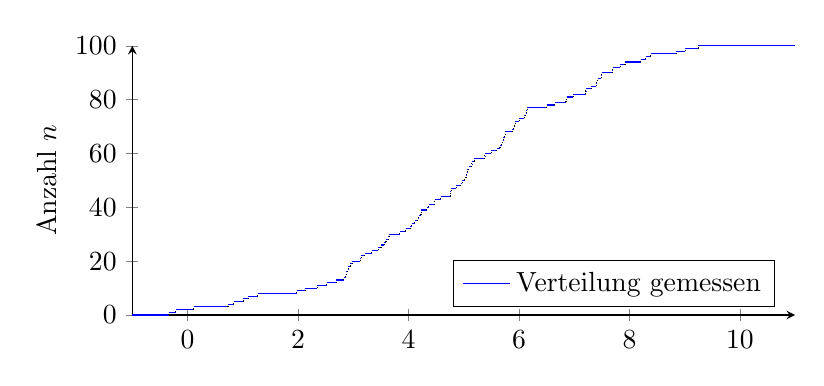
\begin{tikzpicture}
        %note that you have to define \valvarianz and \valoverliney before!
\def\muval{\valoverliney}
\def\sigmaval{\valvarianz}

\begin{axis}[
    domain=-4:14,
    axis x line=bottom, % no box around the plot, only x and y axis
    axis y line=left, % the * would suppress the arrow tips
    ylabel={Anzahl $n$},
    legend pos=south east,
    samples=50,
    height=5cm,
    width=10cm,
    clip=false]

    \ifnum\pdfshellescape=1 %makro to check, if shellescape is set, to prevent errors from windows
    \def\cdf(#1)(#2)(#3){1/2*(1+(erf((#3-#1)/(#2*sqrt(2)))))}
    \addplot[smooth,red] gnuplot{100*\cdf(5)(2)(x)};
    \addlegendentry[align=left]{Verteilung Real};
    \fi

    \addplot[blue] coordinates{(-1, 0)(-0.344732, 0)};
    %-0.344732
    \addlegendentry[align=left]{Verteilung gemessen};
    \addplot[blue,forget plot] coordinates{(-0.344732, 1)(-0.213523, 1)};
    \draw[dotted] (axis cs:-0.344732,0) -- (axis cs: -0.344732, 1);
    %-0.213523
    \addplot[blue,forget plot] coordinates{(-0.213523, 2)(0.109964, 2)};
    \draw[dotted] (axis cs:-0.213523,1) -- (axis cs: -0.213523, 2);
    %0.109964
    \addplot[blue,forget plot] coordinates{(0.109964, 3)(0.732875, 3)};
    \draw[dotted] (axis cs:0.109964,2) -- (axis cs: 0.109964, 3);
    %0.732875
    \addplot[blue,forget plot] coordinates{(0.732875, 4)(0.836437, 4)};
    \draw[dotted] (axis cs:0.732875,3) -- (axis cs: 0.732875, 4);
    %0.836437
    \addplot[blue,forget plot] coordinates{(0.836437, 5)(1.01272, 5)};
    \draw[dotted] (axis cs:0.836437,4) -- (axis cs: 0.836437, 5);
    %1.01272
    \addplot[blue,forget plot] coordinates{(1.01272, 6)(1.09892, 6)};
    \draw[dotted] (axis cs:1.01272,5) -- (axis cs: 1.01272, 6);
    %1.09892
    \addplot[blue,forget plot] coordinates{(1.09892, 7)(1.26684, 7)};
    \draw[dotted] (axis cs:1.09892,6) -- (axis cs: 1.09892, 7);
    %1.26684
    \addplot[blue,forget plot] coordinates{(1.26684, 8)(1.97963, 8)};
    \draw[dotted] (axis cs:1.26684,7) -- (axis cs: 1.26684, 8);
    %1.97963
    \addplot[blue,forget plot] coordinates{(1.97963, 9)(2.12856, 9)};
    \draw[dotted] (axis cs:1.97963,8) -- (axis cs: 1.97963, 9);
    %2.12856
    \addplot[blue,forget plot] coordinates{(2.12856, 10)(2.34886, 10)};
    \draw[dotted] (axis cs:2.12856,9) -- (axis cs: 2.12856, 10);
    %2.34886
    \addplot[blue,forget plot] coordinates{(2.34886, 11)(2.51757, 11)};
    \draw[dotted] (axis cs:2.34886,10) -- (axis cs: 2.34886, 11);
    %2.51757
    \addplot[blue,forget plot] coordinates{(2.51757, 12)(2.69602, 12)};
    \draw[dotted] (axis cs:2.51757,11) -- (axis cs: 2.51757, 12);
    %2.69602
    \addplot[blue,forget plot] coordinates{(2.69602, 13)(2.82636, 13)};
    \draw[dotted] (axis cs:2.69602,12) -- (axis cs: 2.69602, 13);
    %2.82636
    \addplot[blue,forget plot] coordinates{(2.82636, 14)(2.86175, 14)};
    \draw[dotted] (axis cs:2.82636,13) -- (axis cs: 2.82636, 14);
    %2.86175
    \addplot[blue,forget plot] coordinates{(2.86175, 15)(2.87666, 15)};
    \draw[dotted] (axis cs:2.86175,14) -- (axis cs: 2.86175, 15);
    %2.87666
    \addplot[blue,forget plot] coordinates{(2.87666, 16)(2.90335, 16)};
    \draw[dotted] (axis cs:2.87666,15) -- (axis cs: 2.87666, 16);
    %2.90335
    \addplot[blue,forget plot] coordinates{(2.90335, 17)(2.90784, 17)};
    \draw[dotted] (axis cs:2.90335,16) -- (axis cs: 2.90335, 17);
    %2.90784
    \addplot[blue,forget plot] coordinates{(2.90784, 18)(2.94415, 18)};
    \draw[dotted] (axis cs:2.90784,17) -- (axis cs: 2.90784, 18);
    %2.94415
    \addplot[blue,forget plot] coordinates{(2.94415, 19)(2.97867, 19)};
    \draw[dotted] (axis cs:2.94415,18) -- (axis cs: 2.94415, 19);
    %2.97867
    \addplot[blue,forget plot] coordinates{(2.97867, 20)(3.12832, 20)};
    \draw[dotted] (axis cs:2.97867,19) -- (axis cs: 2.97867, 20);
    %3.12832
    \addplot[blue,forget plot] coordinates{(3.12832, 21)(3.14568, 21)};
    \draw[dotted] (axis cs:3.12832,20) -- (axis cs: 3.12832, 21);
    %3.14568
    \addplot[blue,forget plot] coordinates{(3.14568, 22)(3.21075, 22)};
    \draw[dotted] (axis cs:3.14568,21) -- (axis cs: 3.14568, 22);
    %3.21075
    \addplot[blue,forget plot] coordinates{(3.21075, 23)(3.33058, 23)};
    \draw[dotted] (axis cs:3.21075,22) -- (axis cs: 3.21075, 23);
    %3.33058
    \addplot[blue,forget plot] coordinates{(3.33058, 24)(3.45366, 24)};
    \draw[dotted] (axis cs:3.33058,23) -- (axis cs: 3.33058, 24);
    %3.45366
    \addplot[blue,forget plot] coordinates{(3.45366, 25)(3.50146, 25)};
    \draw[dotted] (axis cs:3.45366,24) -- (axis cs: 3.45366, 25);
    %3.50146
    \addplot[blue,forget plot] coordinates{(3.50146, 26)(3.56306, 26)};
    \draw[dotted] (axis cs:3.50146,25) -- (axis cs: 3.50146, 26);
    %3.56306
    \addplot[blue,forget plot] coordinates{(3.56306, 27)(3.59241, 27)};
    \draw[dotted] (axis cs:3.56306,26) -- (axis cs: 3.56306, 27);
    %3.59241
    \addplot[blue,forget plot] coordinates{(3.59241, 28)(3.63463, 28)};
    \draw[dotted] (axis cs:3.59241,27) -- (axis cs: 3.59241, 28);
    %3.63463
    \addplot[blue,forget plot] coordinates{(3.63463, 29)(3.65456, 29)};
    \draw[dotted] (axis cs:3.63463,28) -- (axis cs: 3.63463, 29);
    %3.65456
    \addplot[blue,forget plot] coordinates{(3.65456, 30)(3.83962, 30)};
    \draw[dotted] (axis cs:3.65456,29) -- (axis cs: 3.65456, 30);
    %3.83962
    \addplot[blue,forget plot] coordinates{(3.83962, 31)(3.94673, 31)};
    \draw[dotted] (axis cs:3.83962,30) -- (axis cs: 3.83962, 31);
    %3.94673
    \addplot[blue,forget plot] coordinates{(3.94673, 32)(4.03131, 32)};
    \draw[dotted] (axis cs:3.94673,31) -- (axis cs: 3.94673, 32);
    %4.03131
    \addplot[blue,forget plot] coordinates{(4.03131, 33)(4.05808, 33)};
    \draw[dotted] (axis cs:4.03131,32) -- (axis cs: 4.03131, 33);
    %4.05808
    \addplot[blue,forget plot] coordinates{(4.05808, 34)(4.11354, 34)};
    \draw[dotted] (axis cs:4.05808,33) -- (axis cs: 4.05808, 34);
    %4.11354
    \addplot[blue,forget plot] coordinates{(4.11354, 35)(4.16419, 35)};
    \draw[dotted] (axis cs:4.11354,34) -- (axis cs: 4.11354, 35);
    %4.16419
    \addplot[blue,forget plot] coordinates{(4.16419, 36)(4.18878, 36)};
    \draw[dotted] (axis cs:4.16419,35) -- (axis cs: 4.16419, 36);
    %4.18878
    \addplot[blue,forget plot] coordinates{(4.18878, 37)(4.22557, 37)};
    \draw[dotted] (axis cs:4.18878,36) -- (axis cs: 4.18878, 37);
    %4.22557
    \addplot[blue,forget plot] coordinates{(4.22557, 38)(4.23323, 38)};
    \draw[dotted] (axis cs:4.22557,37) -- (axis cs: 4.22557, 38);
    %4.23323
    \addplot[blue,forget plot] coordinates{(4.23323, 39)(4.33356, 39)};
    \draw[dotted] (axis cs:4.23323,38) -- (axis cs: 4.23323, 39);
    %4.33356
    \addplot[blue,forget plot] coordinates{(4.33356, 40)(4.36949, 40)};
    \draw[dotted] (axis cs:4.33356,39) -- (axis cs: 4.33356, 40);
    %4.36949
    \addplot[blue,forget plot] coordinates{(4.36949, 41)(4.46429, 41)};
    \draw[dotted] (axis cs:4.36949,40) -- (axis cs: 4.36949, 41);
    %4.46429
    \addplot[blue,forget plot] coordinates{(4.46429, 42)(4.47114, 42)};
    \draw[dotted] (axis cs:4.46429,41) -- (axis cs: 4.46429, 42);
    %4.47114
    \addplot[blue,forget plot] coordinates{(4.47114, 43)(4.58031, 43)};
    \draw[dotted] (axis cs:4.47114,42) -- (axis cs: 4.47114, 43);
    %4.58031
    \addplot[blue,forget plot] coordinates{(4.58031, 44)(4.75607, 44)};
    \draw[dotted] (axis cs:4.58031,43) -- (axis cs: 4.58031, 44);
    %4.75607
    \addplot[blue,forget plot] coordinates{(4.75607, 45)(4.75648, 45)};
    \draw[dotted] (axis cs:4.75607,44) -- (axis cs: 4.75607, 45);
    %4.75648
    \addplot[blue,forget plot] coordinates{(4.75648, 46)(4.77195, 46)};
    \draw[dotted] (axis cs:4.75648,45) -- (axis cs: 4.75648, 46);
    %4.77195
    \addplot[blue,forget plot] coordinates{(4.77195, 47)(4.86651, 47)};
    \draw[dotted] (axis cs:4.77195,46) -- (axis cs: 4.77195, 47);
    %4.86651
    \addplot[blue,forget plot] coordinates{(4.86651, 48)(4.94548, 48)};
    \draw[dotted] (axis cs:4.86651,47) -- (axis cs: 4.86651, 48);
    %4.94548
    \addplot[blue,forget plot] coordinates{(4.94548, 49)(4.97367, 49)};
    \draw[dotted] (axis cs:4.94548,48) -- (axis cs: 4.94548, 49);
    %4.97367
    \addplot[blue,forget plot] coordinates{(4.97367, 50)(5.01479, 50)};
    \draw[dotted] (axis cs:4.97367,49) -- (axis cs: 4.97367, 50);
    %5.01479
    \addplot[blue,forget plot] coordinates{(5.01479, 51)(5.04024, 51)};
    \draw[dotted] (axis cs:5.01479,50) -- (axis cs: 5.01479, 51);
    %5.04024
    \addplot[blue,forget plot] coordinates{(5.04024, 52)(5.05053, 52)};
    \draw[dotted] (axis cs:5.04024,51) -- (axis cs: 5.04024, 52);
    %5.05053
    \addplot[blue,forget plot] coordinates{(5.05053, 53)(5.06721, 53)};
    \draw[dotted] (axis cs:5.05053,52) -- (axis cs: 5.05053, 53);
    %5.06721
    \addplot[blue,forget plot] coordinates{(5.06721, 54)(5.09296, 54)};
    \draw[dotted] (axis cs:5.06721,53) -- (axis cs: 5.06721, 54);
    %5.09296
    \addplot[blue,forget plot] coordinates{(5.09296, 55)(5.14038, 55)};
    \draw[dotted] (axis cs:5.09296,54) -- (axis cs: 5.09296, 55);
    %5.14038
    \addplot[blue,forget plot] coordinates{(5.14038, 56)(5.14454, 56)};
    \draw[dotted] (axis cs:5.14038,55) -- (axis cs: 5.14038, 56);
    %5.14454
    \addplot[blue,forget plot] coordinates{(5.14454, 57)(5.1917, 57)};
    \draw[dotted] (axis cs:5.14454,56) -- (axis cs: 5.14454, 57);
    %5.1917
    \addplot[blue,forget plot] coordinates{(5.1917, 58)(5.37826, 58)};
    \draw[dotted] (axis cs:5.1917,57) -- (axis cs: 5.1917, 58);
    %5.37826
    \addplot[blue,forget plot] coordinates{(5.37826, 59)(5.38223, 59)};
    \draw[dotted] (axis cs:5.37826,58) -- (axis cs: 5.37826, 59);
    %5.38223
    \addplot[blue,forget plot] coordinates{(5.38223, 60)(5.49433, 60)};
    \draw[dotted] (axis cs:5.38223,59) -- (axis cs: 5.38223, 60);
    %5.49433
    \addplot[blue,forget plot] coordinates{(5.49433, 61)(5.59523, 61)};
    \draw[dotted] (axis cs:5.49433,60) -- (axis cs: 5.49433, 61);
    %5.59523
    \addplot[blue,forget plot] coordinates{(5.59523, 62)(5.65684, 62)};
    \draw[dotted] (axis cs:5.59523,61) -- (axis cs: 5.59523, 62);
    %5.65684
    \addplot[blue,forget plot] coordinates{(5.65684, 63)(5.69119, 63)};
    \draw[dotted] (axis cs:5.65684,62) -- (axis cs: 5.65684, 63);
    %5.69119
    \addplot[blue,forget plot] coordinates{(5.69119, 64)(5.7074, 64)};
    \draw[dotted] (axis cs:5.69119,63) -- (axis cs: 5.69119, 64);
    %5.7074
    \addplot[blue,forget plot] coordinates{(5.7074, 65)(5.71321, 65)};
    \draw[dotted] (axis cs:5.7074,64) -- (axis cs: 5.7074, 65);
    %5.71321
    \addplot[blue,forget plot] coordinates{(5.71321, 66)(5.74344, 66)};
    \draw[dotted] (axis cs:5.71321,65) -- (axis cs: 5.71321, 66);
    %5.74344
    \addplot[blue,forget plot] coordinates{(5.74344, 67)(5.75382, 67)};
    \draw[dotted] (axis cs:5.74344,66) -- (axis cs: 5.74344, 67);
    %5.75382
    \addplot[blue,forget plot] coordinates{(5.75382, 68)(5.87535, 68)};
    \draw[dotted] (axis cs:5.75382,67) -- (axis cs: 5.75382, 68);
    %5.87535
    \addplot[blue,forget plot] coordinates{(5.87535, 69)(5.90114, 69)};
    \draw[dotted] (axis cs:5.87535,68) -- (axis cs: 5.87535, 69);
    %5.90114
    \addplot[blue,forget plot] coordinates{(5.90114, 70)(5.91929, 70)};
    \draw[dotted] (axis cs:5.90114,69) -- (axis cs: 5.90114, 70);
    %5.91929
    \addplot[blue,forget plot] coordinates{(5.91929, 71)(5.93672, 71)};
    \draw[dotted] (axis cs:5.91929,70) -- (axis cs: 5.91929, 71);
    %5.93672
    \addplot[blue,forget plot] coordinates{(5.93672, 72)(6.00166, 72)};
    \draw[dotted] (axis cs:5.93672,71) -- (axis cs: 5.93672, 72);
    %6.00166
    \addplot[blue,forget plot] coordinates{(6.00166, 73)(6.09481, 73)};
    \draw[dotted] (axis cs:6.00166,72) -- (axis cs: 6.00166, 73);
    %6.09481
    \addplot[blue,forget plot] coordinates{(6.09481, 74)(6.12288, 74)};
    \draw[dotted] (axis cs:6.09481,73) -- (axis cs: 6.09481, 74);
    %6.12288
    \addplot[blue,forget plot] coordinates{(6.12288, 75)(6.13229, 75)};
    \draw[dotted] (axis cs:6.12288,74) -- (axis cs: 6.12288, 75);
    %6.13229
    \addplot[blue,forget plot] coordinates{(6.13229, 76)(6.15318, 76)};
    \draw[dotted] (axis cs:6.13229,75) -- (axis cs: 6.13229, 76);
    %6.15318
    \addplot[blue,forget plot] coordinates{(6.15318, 77)(6.49903, 77)};
    \draw[dotted] (axis cs:6.15318,76) -- (axis cs: 6.15318, 77);
    %6.49903
    \addplot[blue,forget plot] coordinates{(6.49903, 78)(6.65007, 78)};
    \draw[dotted] (axis cs:6.49903,77) -- (axis cs: 6.49903, 78);
    %6.65007
    \addplot[blue,forget plot] coordinates{(6.65007, 79)(6.85014, 79)};
    \draw[dotted] (axis cs:6.65007,78) -- (axis cs: 6.65007, 79);
    %6.85014
    \addplot[blue,forget plot] coordinates{(6.85014, 80)(6.86014, 80)};
    \draw[dotted] (axis cs:6.85014,79) -- (axis cs: 6.85014, 80);
    %6.86014
    \addplot[blue,forget plot] coordinates{(6.86014, 81)(6.98181, 81)};
    \draw[dotted] (axis cs:6.86014,80) -- (axis cs: 6.86014, 81);
    %6.98181
    \addplot[blue,forget plot] coordinates{(6.98181, 82)(7.20432, 82)};
    \draw[dotted] (axis cs:6.98181,81) -- (axis cs: 6.98181, 82);
    %7.20432
    \addplot[blue,forget plot] coordinates{(7.20432, 83)(7.2094, 83)};
    \draw[dotted] (axis cs:7.20432,82) -- (axis cs: 7.20432, 83);
    %7.2094
    \addplot[blue,forget plot] coordinates{(7.2094, 84)(7.30836, 84)};
    \draw[dotted] (axis cs:7.2094,83) -- (axis cs: 7.2094, 84);
    %7.30836
    \addplot[blue,forget plot] coordinates{(7.30836, 85)(7.39552, 85)};
    \draw[dotted] (axis cs:7.30836,84) -- (axis cs: 7.30836, 85);
    %7.39552
    \addplot[blue,forget plot] coordinates{(7.39552, 86)(7.40688, 86)};
    \draw[dotted] (axis cs:7.39552,85) -- (axis cs: 7.39552, 86);
    %7.40688
    \addplot[blue,forget plot] coordinates{(7.40688, 87)(7.42305, 87)};
    \draw[dotted] (axis cs:7.40688,86) -- (axis cs: 7.40688, 87);
    %7.42305
    \addplot[blue,forget plot] coordinates{(7.42305, 88)(7.4921, 88)};
    \draw[dotted] (axis cs:7.42305,87) -- (axis cs: 7.42305, 88);
    %7.4921
    \addplot[blue,forget plot] coordinates{(7.4921, 89)(7.49466, 89)};
    \draw[dotted] (axis cs:7.4921,88) -- (axis cs: 7.4921, 89);
    %7.49466
    \addplot[blue,forget plot] coordinates{(7.49466, 90)(7.69063, 90)};
    \draw[dotted] (axis cs:7.49466,89) -- (axis cs: 7.49466, 90);
    %7.69063
    \addplot[blue,forget plot] coordinates{(7.69063, 91)(7.694, 91)};
    \draw[dotted] (axis cs:7.69063,90) -- (axis cs: 7.69063, 91);
    %7.694
    \addplot[blue,forget plot] coordinates{(7.694, 92)(7.83635, 92)};
    \draw[dotted] (axis cs:7.694,91) -- (axis cs: 7.694, 92);
    %7.83635
    \addplot[blue,forget plot] coordinates{(7.83635, 93)(7.91892, 93)};
    \draw[dotted] (axis cs:7.83635,92) -- (axis cs: 7.83635, 93);
    %7.91892
    \addplot[blue,forget plot] coordinates{(7.91892, 94)(8.20621, 94)};
    \draw[dotted] (axis cs:7.91892,93) -- (axis cs: 7.91892, 94);
    %8.20621
    \addplot[blue,forget plot] coordinates{(8.20621, 95)(8.29379, 95)};
    \draw[dotted] (axis cs:8.20621,94) -- (axis cs: 8.20621, 95);
    %8.29379
    \addplot[blue,forget plot] coordinates{(8.29379, 96)(8.38558, 96)};
    \draw[dotted] (axis cs:8.29379,95) -- (axis cs: 8.29379, 96);
    %8.38558
    \addplot[blue,forget plot] coordinates{(8.38558, 97)(8.84879, 97)};
    \draw[dotted] (axis cs:8.38558,96) -- (axis cs: 8.38558, 97);
    %8.84879
    \addplot[blue,forget plot] coordinates{(8.84879, 98)(9.00956, 98)};
    \draw[dotted] (axis cs:8.84879,97) -- (axis cs: 8.84879, 98);
    %9.00956
    \addplot[blue,forget plot] coordinates{(9.00956, 99)(9.24935, 99)};
    \draw[dotted] (axis cs:9.00956,98) -- (axis cs: 9.00956, 99);
    %9.24935
    \addplot[blue,forget plot] coordinates{(9.24935, 100)(11, 100)};
    \draw[dotted] (axis cs:9.24935,99) -- (axis cs: 9.24935, 100);
\end{axis}
%Graphic
    \end{tikzpicture}
    \caption{Zu Beispiel \ref{bsp:messwerte_t_berechnung}: Verteilung der Messwerte.}
    \label{fig:normaldist_messwerte}
\end{figure}

\begin{figure}
    \centering
    \begin{tikzpicture}
        {
\def\muval{\valoverliney}
\def\sigmaval{\valvarianz}
\def\tauval{1.96}
\def\beginval{-2}
\def\endval{12}
\begin{axis}[
    domain=\beginval:\endval,
    axis x line=bottom, % no box around the plot, only x and y axis
    axis y line=left, % the * would suppress the arrow tips
    xtick={0,2,4,6,8,10},
    ylabel={Wahrscheinlichkeit $p$},
    y tick label style={/pgf/number format/fixed},
    samples=50,
    height=5cm,
    width=10cm,
    clip=false
]

% Fill curve-part left
\addplot [
    fill=brown!50,
    draw=none,
    forget plot,            %prevent from listing in legend
    domain=\beginval:\ttwenty
] {normal_distribution(\muval,\sigmaval,x)} \closedcycle;

% Fill curve-part left
\addplot [
    fill=red!50,
    draw=none,
    forget plot,            %prevent from listing in legend
    domain=\ttwenty:\tfourty
] {normal_distribution(\muval,\sigmaval,x)} \closedcycle;

% Fill curve-part middle
\addplot [
    fill=yellow!50,
    draw=none,
    forget plot,            %prevent from listing in legend
    domain=\tfourty:\tsixty
] {normal_distribution(\muval,\sigmaval,x)} \closedcycle;

% Fill curve-part middle
\addplot [
    fill=orange!50,
    draw=none,
    forget plot,            %prevent from listing in legend
    domain=\tsixty:\teighty
] {normal_distribution(\muval,\sigmaval,x)} \closedcycle;

% Fill curve-part middle
\addplot [
    fill=blue!50,
    draw=none,
    forget plot,            %prevent from listing in legend
    domain=\teighty:\endval
] {normal_distribution(\muval,\sigmaval,x)} \closedcycle;

% Draw curves
\addplot [thin, smooth, color=green, name path global=plot] {normal_distribution(\muval,\sigmaval,x)};

%find intersection with normal_distribution on theta=\muval-\tauval
\node[coordinate] (Ref) at (axis cs:\ttwenty,0) {};
\path[name path global=RefPath] (Ref |- current axis.south) -- (Ref |- current axis.north);
\path [name intersections={of=plot and RefPath}];
\coordinate (I3)  at (intersection-1);
%draw line to intersection on theta=\muval-\tauval
\draw [ultra thick,dashed,red] (I3) -- ({rel axis cs:0,0}-|Ref)
    node [above left,black] {$k_1$};

%find intersection with normal_distribution on theta=\muval-\tauval
\node[coordinate] (Ref) at (axis cs:\ttwenty,0) {};
\path[name path global=RefPath] (Ref |- current axis.south) -- (Ref |- current axis.north);
\path [name intersections={of=plot and RefPath}];
\coordinate (I3)  at (intersection-1);
%draw line to intersection on theta=\muval-\tauval
\draw [ultra thick,dashed,red] (I3) -- ({rel axis cs:0,0}-|Ref)
    node [above right,black] {$k_2$};

%find intersection with normal_distribution on theta=\muval-\tauval
\node[coordinate] (Ref) at (axis cs:\tfourty,0) {};
\path[name path global=RefPath] (Ref |- current axis.south) -- (Ref |- current axis.north);
\path [name intersections={of=plot and RefPath}];
\coordinate (I3)  at (intersection-1);
%draw line to intersection on theta=\muval-\tauval
\draw [ultra thick,dashed,red] (I3) -- ({rel axis cs:0,0}-|Ref)
    node [above right,black] {$k_3$};

%find intersection with normal_distribution on theta=\muval-\tauval
\node[coordinate] (Ref) at (axis cs:\tsixty,0) {};
\path[name path global=RefPath] (Ref |- current axis.south) -- (Ref |- current axis.north);
\path [name intersections={of=plot and RefPath}];
\coordinate (I3)  at (intersection-1);
%draw line to intersection on theta=\muval-\tauval
\draw [ultra thick,dashed,red] (I3) -- ({rel axis cs:0,0}-|Ref)
    node [above right,black] {$k_4$};

%find intersection with normal_distribution on theta=\muval-\tauval
\node[coordinate] (Ref) at (axis cs:\teighty,0) {};
\path[name path global=RefPath] (Ref |- current axis.south) -- (Ref |- current axis.north);
\path [name intersections={of=plot and RefPath}];
\coordinate (I3)  at (intersection-1);
%draw line to intersection on theta=\muval-\tauval
\draw [ultra thick,dashed,red] (I3) -- ({rel axis cs:0,0}-|Ref)
    node [above right,black] {$k_5$};

\end{axis}
}
%Graphic
    \end{tikzpicture}
    \caption{Zu Beispiel \ref{bsp:messwerte_t_berechnung}: Verteilung der Klassen, jede hat 20\% Wahrscheinlichkeit.}
    \label{fig:classes}
\end{figure}

\begin{table}
    \centering
    \begin{tabular}{|c|c|c|c|}
        \hline
        $i$ & $y_i$ & $np_i$ & $\frac{(y_i-np_i)^2}{np_i}$\\
        \hline
        $1$ & $\numca$ & $\frac{\valn}{\valk}=\tnoverk$ & $\frac{(\numca-\tnoverk)^2}{\tnoverk}=\frac{\tvalcanumerator}{\tnoverk}$ \\
        \hline
        $2$ & $\numcb$ & $\frac{\valn}{\valk}=\tnoverk$ & $\frac{(\numcb-\tnoverk)^2}{\tnoverk}=\frac{\tvalcbnumerator}{\tnoverk}$ \\
        \hline
        $3$ & $\numcc$ & $\frac{\valn}{\valk}=\tnoverk$ & $\frac{(\numcc-\tnoverk)^2}{\tnoverk}=\frac{\tvalccnumerator}{\tnoverk}$ \\
        \hline
        $4$ & $\numcd$ & $\frac{\valn}{\valk}=\tnoverk$ & $\frac{(\numcd-\tnoverk)^2}{\tnoverk}=\frac{\tvalcdnumerator}{\tnoverk}$ \\
        \hline
        $5$ & $\numce$ & $\frac{\valn}{\valk}=\tnoverk$ & $\frac{(\numce-\tnoverk)^2}{\tnoverk}=\frac{\tvalcenumerator}{\tnoverk}$ \\
        \hline
        & & $\sum_{j=1}^k$ & $\frac{\tvalcanumerator+\tvalcbnumerator+\tvalccnumerator+\tvalcdnumerator+\tvalcenumerator}{\tnoverk}=\frac{\tvalnumerator}{\tnoverk}=\tval$\\
        \hline
    \end{tabular}
    \caption{Berechnung von $T=\sum_{j=1}^k\frac{(y_i-np_i)^2}{np_i}$ (siehe Beispiel \ref{bsp:messwerte_t_berechnung})}\label{tab:messwerte_t_berechnung}
\end{table}
}

\index{Anpassungstests|)}
\subsection{Tests und Konfidenzintervalle}\index{Konfidenzintervall!Tests}
Es gibt einen interessanten Zusammenhang zwischen Tests und Konfidenzintervallen:

\begin{satz} \textbf{Dualität von Konfidenzintervall und Tests}\index{Dualität Konfidenzintervall/Tests}\index{Konfidenzintervall!Dualität mit Tests|see{Dualität Konfidenzintervall/Tests}}\index{Tests!Dualität mit Konfidenzintervall|see{Dualität Konfidenzintervall/Tests}}\\
Wenn $I=[a(X_1,\dots, X_n),b(X_1,\dots, X_n)]$ ein Konfidenzintervall (mit Übergangswahrscheinlichkeit $\gamma=1-\alpha$) für einen Parameter $\theta$ ist, dann erhält man einen Test mit Signifikanzniveau $\alpha$, wenn man die Nullhypothese $H_0:\theta=\theta_0$ genau dann verwift, wenn $\theta_0\not\in I$''.\\

Ist umgekehrt für jedes $\theta_0$ ein Test mit Niveau $\alpha$
für die Nullhypothese $H_0:\theta=\theta_0$ gegeben, dann ist
die Menge aller $\theta_0$, für die $H_0:\theta=\theta_0$ 
nicht verworfen wird, ein Konfidenzintervall (mit 
Überdeckungswahrscheinlichkeit $\gamma=1-\alpha$).
\end{satz}
\begin{bsp}
{
    \def\xquer{0.89}
    \def\snval{0.26}
    \def\nval{51}
    \def\alphaval{5}
    \def\tval{2.01}
    \pgfmathsetmacro{\fractionval}{\snval/sqrt(\nval)}
    \pgfmathsetmacro{\productval}{\tval*\fractionval}
    \pgfmathsetmacro{\leftval}{\xquer-\productval}
    \pgfmathsetmacro{\rightval}{\xquer+\productval}
Rufen wir uns nochmal das Beispiel mit der lügenden Obstverkäuferin ins Gedächtnis:
\ref{bsp:konfidenzintervall} bzw. die Fortsetzung \ref{bsp:test_sigma_unbekannt}, denn beide sind ein Beispiel für die Dualität von Konfidenzintervall und Test.

    Wir haben beispielsweise $\mu_0=1$ und $\mu_0=0.75$ verworfen, aber $\mu_0=0.9$ angenommen. Genau dieses Verhalten spiegelt sich auch im Konfidenzintervall wieder, denn es lautete: $KI=[\leftval,\rightval]$.

}
\end{bsp}
\index{Tests|)}
\index{Statistik|)}
